\documentclass[letterpaper]{article}\usepackage[]{graphicx}\usepackage[]{color}
%% maxwidth is the original width if it is less than linewidth
%% otherwise use linewidth (to make sure the graphics do not exceed the margin)
\makeatletter
\def\maxwidth{ %
  \ifdim\Gin@nat@width>\linewidth
    \linewidth
  \else
    \Gin@nat@width
  \fi
}
\makeatother

\definecolor{fgcolor}{rgb}{0.345, 0.345, 0.345}
\newcommand{\hlnum}[1]{\textcolor[rgb]{0.686,0.059,0.569}{#1}}%
\newcommand{\hlstr}[1]{\textcolor[rgb]{0.192,0.494,0.8}{#1}}%
\newcommand{\hlcom}[1]{\textcolor[rgb]{0.678,0.584,0.686}{\textit{#1}}}%
\newcommand{\hlopt}[1]{\textcolor[rgb]{0,0,0}{#1}}%
\newcommand{\hlstd}[1]{\textcolor[rgb]{0.345,0.345,0.345}{#1}}%
\newcommand{\hlkwa}[1]{\textcolor[rgb]{0.161,0.373,0.58}{\textbf{#1}}}%
\newcommand{\hlkwb}[1]{\textcolor[rgb]{0.69,0.353,0.396}{#1}}%
\newcommand{\hlkwc}[1]{\textcolor[rgb]{0.333,0.667,0.333}{#1}}%
\newcommand{\hlkwd}[1]{\textcolor[rgb]{0.737,0.353,0.396}{\textbf{#1}}}%
\let\hlipl\hlkwb

\usepackage{framed}
\makeatletter
\newenvironment{kframe}{%
 \def\at@end@of@kframe{}%
 \ifinner\ifhmode%
  \def\at@end@of@kframe{\end{minipage}}%
  \begin{minipage}{\columnwidth}%
 \fi\fi%
 \def\FrameCommand##1{\hskip\@totalleftmargin \hskip-\fboxsep
 \colorbox{shadecolor}{##1}\hskip-\fboxsep
     % There is no \\@totalrightmargin, so:
     \hskip-\linewidth \hskip-\@totalleftmargin \hskip\columnwidth}%
 \MakeFramed {\advance\hsize-\width
   \@totalleftmargin\z@ \linewidth\hsize
   \@setminipage}}%
 {\par\unskip\endMakeFramed%
 \at@end@of@kframe}
\makeatother

\definecolor{shadecolor}{rgb}{.97, .97, .97}
\definecolor{messagecolor}{rgb}{0, 0, 0}
\definecolor{warningcolor}{rgb}{1, 0, 1}
\definecolor{errorcolor}{rgb}{1, 0, 0}
\newenvironment{knitrout}{}{} % an empty environment to be redefined in TeX

\usepackage{alltt}
\pdfpagewidth 8.5in
\pdfpageheight 11.0in

\usepackage{ucs}
\usepackage[utf8x]{inputenc}
\newcommand{\HRule}{\rule{\linewidth}{0.5mm}}


\usepackage[hmargin=3cm,vmargin=3.5cm]{geometry}
\usepackage{ucs}
\usepackage[utf8x]{inputenc}
\usepackage{amsmath}
\usepackage{amsfonts}
\usepackage{dcolumn}
\usepackage{fancyhdr}
\usepackage{amssymb}
\usepackage{hyperref}
\usepackage[justification=centering]{caption}
\usepackage{enumerate}
\usepackage{varioref}
\usepackage{graphicx}
\usepackage{cancel}
\usepackage{pbox}
\newcounter{exer}
\numberwithin{exer}{section}
\usepackage{color}
\usepackage{dirtytalk}
\usepackage{array}
\newcolumntype{P}[1]{>{\centering\arraybackslash}p{#1}}
\usepackage[round]{natbib}
\bibliographystyle{plainnat}

\pagestyle{fancyplain}
\usepackage{lastpage}
\definecolor{hellgrau2}{gray}{.6}
\renewcommand{\headrulewidth}{0pt}
\renewcommand{\footrulewidth}{1pt \color{hellgrau2}}
\newcommand{\co}{CO\ensuremath{_2} }
\fancyfoot{}
\fancyhf{}
\rfoot{\textbf{Page \thepage\ of \pageref{LastPage}}}
 \lfoot{\textbf{ECON 204: Conteporary Economic Issues}}
 \cfoot{\textbf{}}

\usepackage{mdframed}
\usepackage{ntheorem}
\theoremstyle{nonumberplain}
\theorembodyfont{\upshape}
\definecolor{bisque}{rgb}{1.0, 0.89, 0.77}
\definecolor{etonblue}{rgb}{0.59, 0.78, 0.64}
\definecolor{blizzardblue}{rgb}{0.67, 0.9, 0.93}
\definecolor{cornsilk}{rgb}{1.0, 0.97, 0.86}
\definecolor{banana}{rgb}{0.98, 0.91, 0.71}
\newmdtheoremenv[leftmargin=20, rightmargin=20,backgroundcolor=bisque,ntheorem]{background}{Background Information}
\newmdtheoremenv[leftmargin=20, rightmargin=20,backgroundcolor=etonblue,ntheorem]{important}{Important}
\newmdtheoremenv[leftmargin=20, rightmargin=20,backgroundcolor=cornsilk,ntheorem]{anime}{Suggested Animation}
\newmdtheoremenv[leftmargin=20, rightmargin=20,backgroundcolor=banana,ntheorem]{pause}{Pause \& Practice}
\newmdtheoremenv[leftmargin=20, rightmargin=20,backgroundcolor=bisque,ntheorem]{devel}{Note to the developers}
\usepackage{soul}
\newcommand{\mathcolorbox}[1]{\colorbox{blizzardblue}{$\displaystyle #1$}}
\IfFileExists{upquote.sty}{\usepackage{upquote}}{}
\begin{document}
\noindent
 \textsc{\Large \textbf{Income Inequality}}\\[.1cm]
 \begin{center}
   \line(1,0){450}\\[0.2cm]
   \end{center}


\tableofcontents

\section{Introduction}\label{sec:intro}
In this part of the course you will learn how to define and measure income
inequality and poverty. The focus is on analyzing the evolution of
inequality and poverty by individual characteristics in Canada and to
compare Canada with other countries. Also, you will analyze the
comovement between inequality, poverty and real per capita GDP.




\subsubsection*{Key Terms}
  
\begin{itemize}
\item \textbf{Decile:} When the population is divided into ten equal
  groups ordered with respect to a variable, the groups are called
  deciles. For example, the first income decile is one tenth (10\%) of
  the population with the lowest income.  
\item \textbf{Economic growth:} This is the growth rate of the real
  per capital GDP.
\item \textbf{Economic mobility:} This characterizes the ability for
  individuals to move from one part of the income distribution to
  another.  
\item \textbf{Gini coefficient:} This is a global measure of
  inequality. It goes from 0 (perfect equality) to 1 (perfect
  inequality). 
\item \textbf{Income share:} This is the proportion of total income
  that goes to an individual or a group. For example, if the income
  share of females is 55\%, it means that 55\% of the total income is
  earned by women.
\item \textbf{Lorenz Curve:} This is a line chart that illustrates the
  cumulative income share of the population as a function of the
  proportion of the population. For example, the points (0.05,0.10)
  and (0.60, 0.50) on the Lorenz curve mean that 10\% of the poorest
  individuals share 5\% of total income of the economy and 50\% share
  60\% of total income.  
\item \textbf{Low income measure (LIM):} This is equal to half the
  median of income. It is one of the measures of the poverty
  line. Individuals with income less than the LIM are considered below
  the poverty line.
\item \textbf{Market basket measure (MBM):} This is the value of a
  basket of goods used in one definition of the poverty
  line. Individuals with income less than the MBM are considered below
  the poverty line.
\item \textbf{Median:} This is a number that separates the
  distribution of a variable in two equal groups. For example, the
  median of income in Canada is \$40,000 if income is less then
  \$40,000 for 50\% of the population and it is higher for the other
  50\%.
\item \textbf{Per capita:} This is a Latin word that means by
  head. For example, the per capita income is the average income by
  individual.
\item \textbf{Quintile:} When the population is divided into five
  equal groups ordered with respect to a variable, the groups are
  called quintiles. For example, the first income quintile is one
  fifth (20\%) of the population with the lowest income.
\end{itemize}

\section{Income Inequality}
\subsection{Economic Growth}

Economic growth is defined as the growth rate of the real per capita
GDP defined as
\[
\mathcolorbox{
\mbox{Real per capita GDP} = \frac{\mbox{Real GDP}}{\mbox{Population}}
  }\,.
\]
Since GDP is also a measure of total income (remember the equivalence
between the three approaches to measure GDP), we also call it average
real per capita income. We start by defining this measure because one
of the purpose of this module is to analyze the relationship between
economic growth and income inequality.

To obtain the real per capita GDP, we need to download the real GDP
\citep*{gdp-expenditure} and the population \citep*{population} series
from Statistics Canada. The population series can be obtained by using
the keyword population and selecting the Population estimates,
quarterly link as in the following screenshot (Canada and Quarterly
was also selected):

\begin{center}
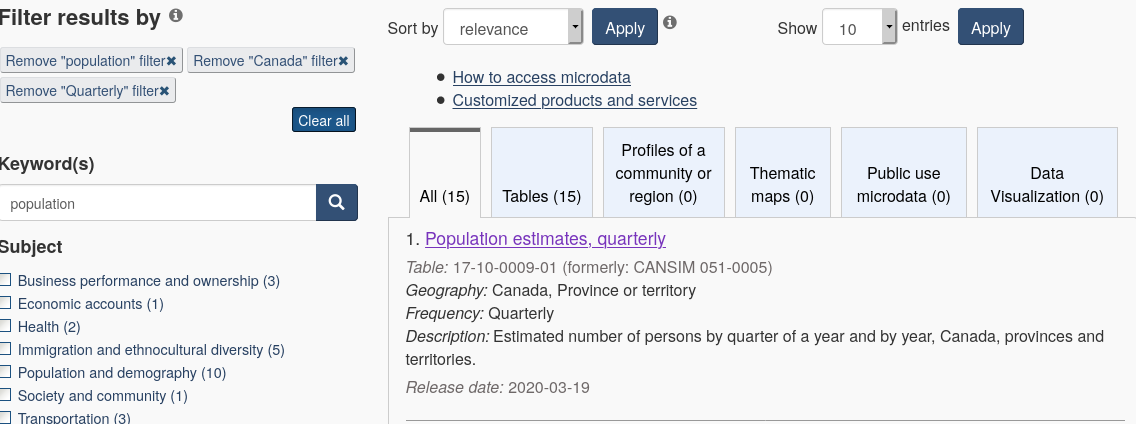
\includegraphics[scale=.25]{week7/pop.png}  
  \end{center}


The following graphs show the low frequency components of the per
capita real GDP (left) and the annualized per capita real GDP growth
rate (right). If you try do reproduce the graphs, by careful with the
units used by Statistics Canada for the GDP and population. In the
tables, population is in units and GDP is in millions. Therefore you
need to express population in millions by dividing the series by one
million before computing the real per capita GDP. You should get, as
we see on the left graph, that the real per capita GDP increased from
20,000 to 55,000 dollars of 2012 between 1961 and 2020. Since its
trending behaviour is roughly constant, it implies a decreasing growth
rate on average as shown by the red dashed line on the right graph.

\begin{center}
\begin{minipage}{.45\textwidth}
\begin{knitrout}\footnotesize
\definecolor{shadecolor}{rgb}{0.969, 0.969, 0.969}\color{fgcolor}
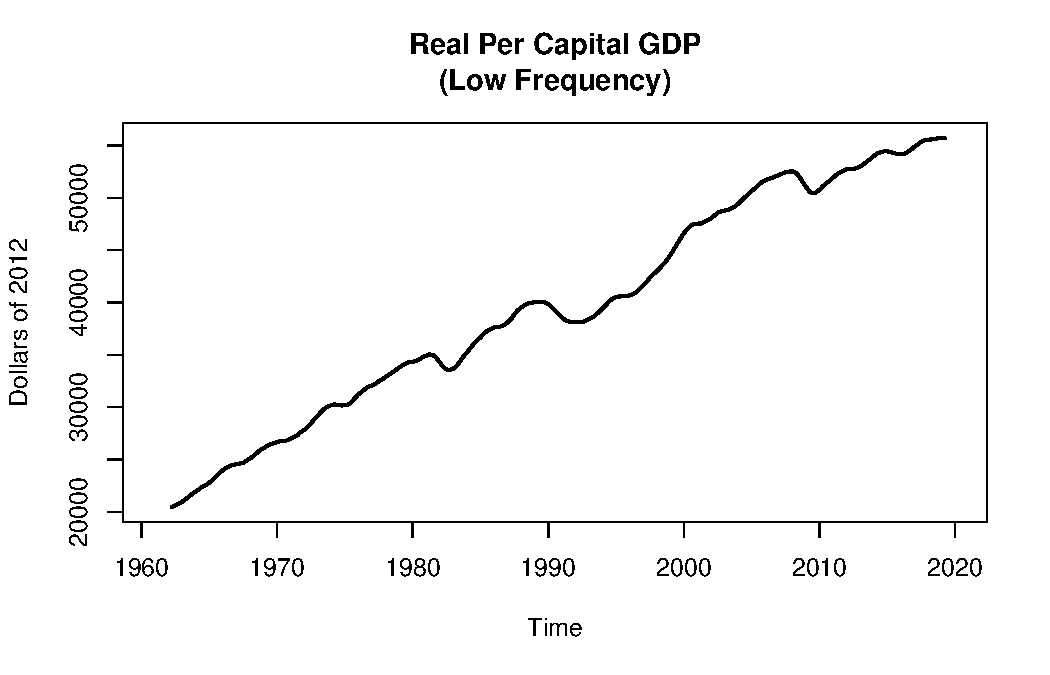
\includegraphics[width=\maxwidth]{week7/week7-growth1-1} 

\end{knitrout}
\end{minipage}
\begin{minipage}{.45\textwidth}
\begin{knitrout}\footnotesize
\definecolor{shadecolor}{rgb}{0.969, 0.969, 0.969}\color{fgcolor}
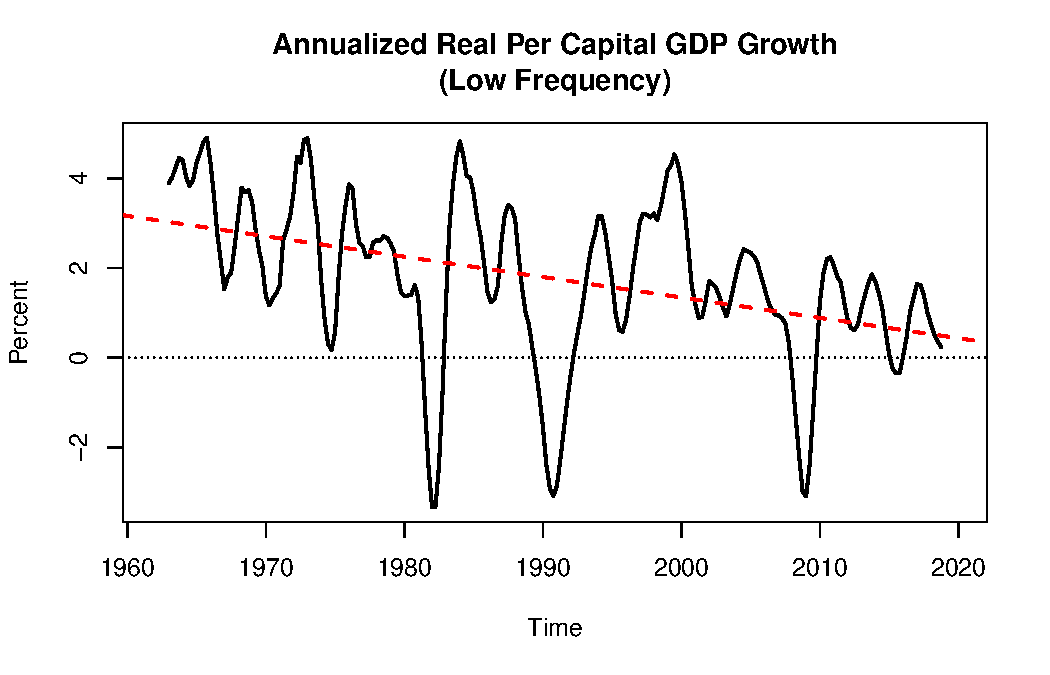
\includegraphics[width=\maxwidth]{week7/week7-growth2-1} 

\end{knitrout}
\end{minipage}
\end{center}
This result implies that Canadians get richer and richer in real terms
on average. Being richer in real terms means that we can buy more
goods. It is therefore a sign that the standard of living of Canadians
has improved over the period on average. However, the result does not
imply that the standard of living of every Canadian has improved. In
this module, we are interested in the allocation of real GDP across
individuals, how the allocation has evolved through time and how it is
related to economic growth. 

\subsection{Measuring Inequality: Income by Quintile}

\subsubsection*{Quintiles}

When we divide the population into five equal groups based on the
distribution of a given variable, the groups are called quintiles. The
lowest quintile represents 20\% of the population with the smallest
values and the fifth quintile includes 20\% of the population with the
highest values. For example, suppose the population is composed of 15
individuals. The following table shows the age and expenditure of each
individual.
\begin{center}
\resizebox{0.9\linewidth}{!}{\begin{tabular}{cccccccccccccccc}
\multicolumn{16}{c}{\textbf{Expenditure and Age by Individual}}\\\hline
Individual&1&2&3&4&5&6&7&8&9&10&11&12&13&14&15\\
Age&19&23&45&18&64&55&34&23&22&44&70&61&49&21&43\\
Expenditure&100&210&80&30&312&190&201&236&341&34&40&101&170&190&343

\\\hline
\end{tabular}}
\end{center}
To construct quintiles according to the age variable, we first sort
individuals by age and divide the population in five equal groups
starting with the youngest and ending with the oldest:
\begin{center}
\resizebox{0.9\linewidth}{!}{\begin{tabular}{cccc|ccc|ccc|ccc|ccc}
 \multicolumn{16}{c}{\textbf{Age Quintiles}}\\\hline
&\multicolumn{3}{c|}{First quintile}&\multicolumn{3}{c|}{Second quintile}
    &\multicolumn{3}{c|}{Third quintile}
    &\multicolumn{3}{c|}{Fourth quintile}
    &\multicolumn{3}{c}{Fifth quintile}\\\hline
Individual&4&1&14&9&2&8&7&15&10&3&13&6&12&5&11\\
Age&18&19&21&22&23&23&34&43&44&45&49&55&61&64&70\\
Expenditure&30&100&190&341&210&236&201&343&34&80&170&190&101&312&40

\\\hline
\end{tabular}}
\end{center}
The individuals that we put in each quintile depends on the
variable. For example, we can see in the following table that if the
quintiles are based on expenditure, they include different
individuals.
\begin{center}
\resizebox{0.9\linewidth}{!}{\begin{tabular}{cccc|ccc|ccc|ccc|ccc}
 \multicolumn{16}{c}{\textbf{Expenditure Quintiles}}\\\hline    
&\multicolumn{3}{c|}{First quintile}&\multicolumn{3}{c|}{Second quintile}
    &\multicolumn{3}{c|}{Third quintile}
    &\multicolumn{3}{c|}{Fourth quintile}
    &\multicolumn{3}{c}{Fifth quintile}\\\hline
Individual&4&10&11&3&1&12&13&14&6&7&2&8&5&9&15\\
Age&18&44&70&45&19&61&49&21&55&34&23&23&64&22&43\\
Expenditure&30&34&40&80&100&101&170&190&190&201&210&236&312&341&343

\\\hline
\end{tabular}}
\end{center}

The purpose of dividing the population into quintiles is to compare
the characteristics of groups of comparable individuals. For example,
we may be interested in comparing the average expenditure by age
quintile. The following table shows the average age and average
expenditure by age quintile. The values are obtained averaging the
values in each quintile. For example the average age and expenditure
for the low age quintile are:

\[
\mbox{Average age (first quintile)} = \frac{1}{3}(18 + 
19 + 21)=19.33
\]
and
\[
\mbox{Average expenditure (first quintile)} = \frac{1}{3}(30 + 
100 + 190)=106.67
\]
\begin{center}
\resizebox{0.9\linewidth}{!}{\begin{tabular}{cccccc}
    \multicolumn{6}{c}{\textbf{Average by Age Quintile}}\\\hline        
&First quintile&Second quintile&Third quintile&Fourth quintile&Fifth quintile\\\hline    
Age&19.33&22.67&40.33&49.67&65\\
Expenditure&106.67&262.33&192.67&146.67&151

\\\hline
\end{tabular}}
\end{center}
First we can compare the average age per quintile: the average age of
the 20\% youngest is 19.33 years and the average for the 20\%
oldest is 65. We can also compare other
characteristics. In the table, we see that the expenditure is the
highest on average in the second age quintile and the lowest in the
first age quintile. Similarly, we can analyze the average by
expenditure quintile:

\[
\mbox{Average age (first quintile)} = \frac{1}{3}(18 + 
44 + 70)=44
\]
and
\[
\mbox{Average expenditure (first quintile)} = \frac{1}{3}(30 + 
34 + 40)=34.67
\]
\begin{center}
\resizebox{0.9\linewidth}{!}{\begin{tabular}{cccccc}
    \multicolumn{6}{c}{\textbf{Average by Expenditure Quintile}}\\\hline        
&First quintile&Second quintile&Third quintile&Fourth quintile&Fifth quintile\\\hline    
Age&44&41.67&41.67&26.67&43\\
Expenditure&34.67&93.67&183.33&215.67&332

\\\hline
\end{tabular}}
\end{center}
We can conclude that the average age for the 20\% of the population
that spend the least is 44 years and it is 43
years for the 20\% of the population that spend the most. Similarly,
the average expenditure for the 20\% of the population that spend the
least is \$34.67 and it is equal to \$332 for the
20\% that spend the most.

Notice that we can divide the population by more than five equal
groups. Other common ways of dividing the population is by deciles and
percentiles. When the population is divided into ten equal groups, the
groups are called deciles and when the population is divided into one
hundred groups, the groups are called percentiles. For example, the
bottom income decile represent 10\% of the population with the lowest
incomes and the top percentile is 1\% of the population with the
highest incomes.

\subsubsection*{Average Income per Quintile in Canada}

Dividing the population in quintiles based on income is one way to
analyze the income distribution. Statistics Canada provides a table in
which the number of households are divided into income quintiles, and
returns several statistics by quintile \citep*{distribution3}. The
following table shows the average household income by income quintile
(first column) and the share of total income (second column). The
first column is obtained by selecting Value per household in the
\textbf{Statistics} tab, the Lowest to Highest income quintiles in the
\textbf{Characteristics} tab and Household disposable income in the
\textbf{Income, consumption and savings} tab of the Statistics Canada
table number 36-10-0587-01. The second column is obtained by replacing
Value per household by Distribution of value in the
\textbf{Statistics} tab (for a specific table enter the table number
as keyword).
\begin{center}
\resizebox{0.9\linewidth}{!}{  
% latex table generated in R 3.6.3 by xtable 1.8-4 package
% Fri Apr 24 16:50:14 2020
\begin{tabular}{lcc}
  \multicolumn{3}{c}{\textbf{Average Income by Quintile in 2018}} \\
 \hline
 & Average Household Income (dollars) & Share of Total Household Income (percent) \\ 
  \hline
First Income Quintile & 23,537 & 5.90 \\ 
  Second Income Quintile & 49,137 & 12.40 \\ 
  Third Income Quintile & 69,943 & 17.60 \\ 
  Fourth Income Quintile & 91,798 & 23.10 \\ 
  Fifth Income Quintile & 162,231 & 40.90 \\ 
   \hline
\end{tabular}

}
\end{center}
Therefore, the average income for the 20\% poorest households is
\$23,537 and it is equal
to \$162,231 for the 20\%
richest households. From the second column, it implies that
5.9\% of total income is allocated to the poorest and
40.9\% of total income is allocated to the richest. We can
also say that 40.9\% of total income goes to 20\% of the
population. We clearly see from this table that total total income is
not allocated equally across household families. 



\subsection{Measuring Inequality: Histograms}

\subsubsection*{Distribution of Income Across Individuals}

To get a better picture of how total income is allocated in the
population, we can create the histogram of income. Creating an
histogram for income requires observations at the individuals, which
is not directly available from the Statistics Canada website. We need
data from the Census of population that can be downloaded from the
Ontario Data Documentation, Extraction Service and Infrastructure
($<$odesi$>$). The website
\href{https://search2.odesi.ca/}{https://search2.odesi.ca/} is
accessible publicly, but the downloads are restricted. As a student,
you are allowed to download the data through the
\href{https://subjectguides.uwaterloo.ca/stats_data}{University
  library}. If you select \textbf{ODESI Data Retrieval} in the Key
Links panel on the left, you will be asked to login with your last
name and Watcard barcode number. Once logged in, you can download any
data files. For this course, you are not required to download the data
from that source because the manipulation of survey and census data is
beyond the score of the course. However, you are welcome for your own
interest to surf on the website. The data used in the following is
from the 2016 census \citep*{census2016}. It is described on the
following screenshot:
\begin{center}
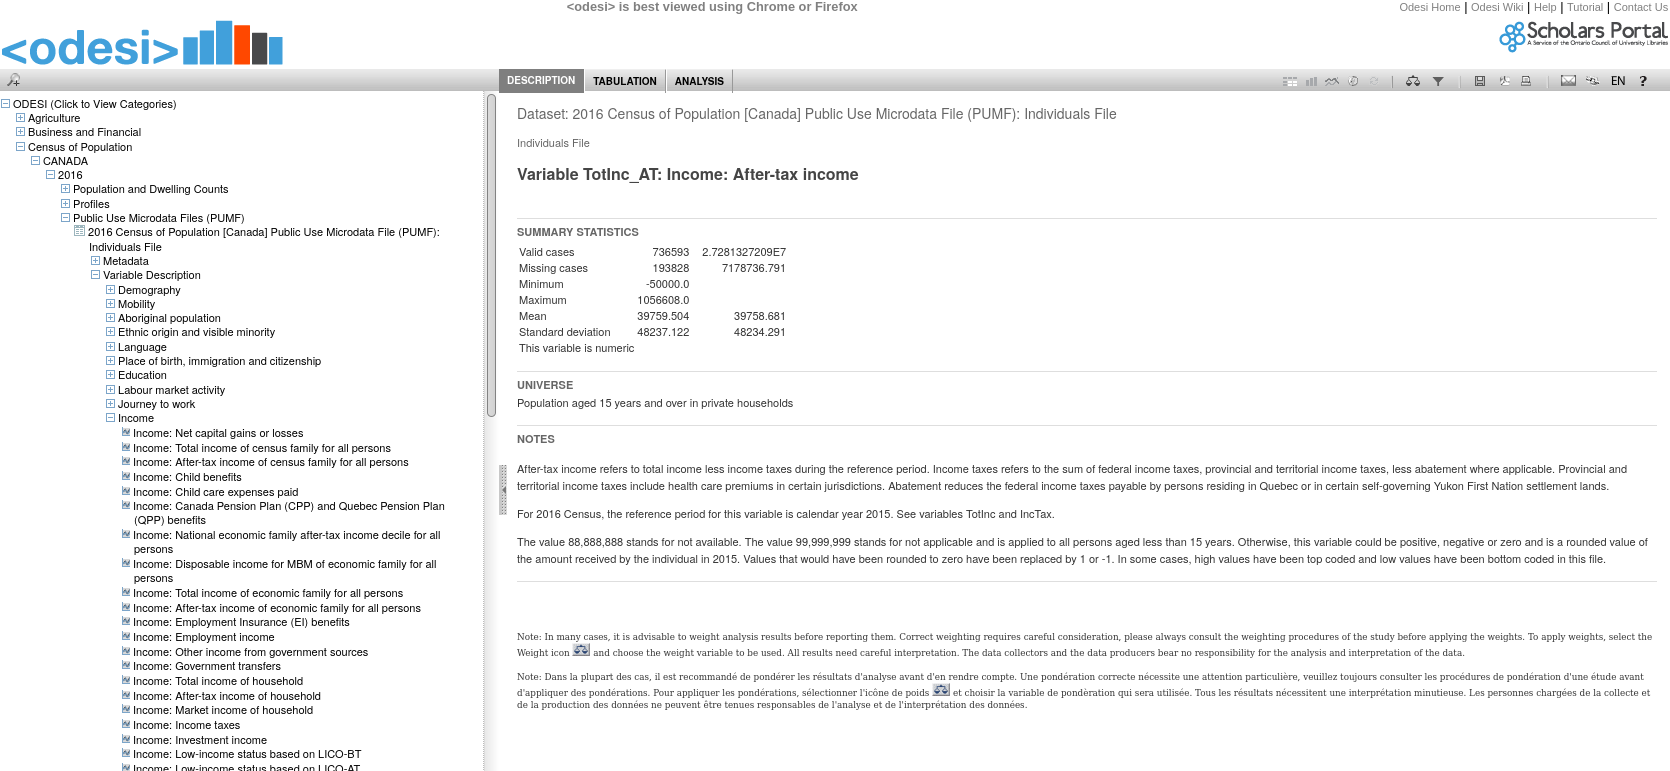
\includegraphics[scale=0.25]{week7/odesi.png}
\end{center}
Without going into too much details, the dataset contains the
after-tax income series of about 735,000 individuals. It is a
representative sample that represents approximately 1/37 of the
Canadian population 15 years and older. Therefore, we have to multiply
the number of counts by 37 to have a sense of how many individuals we
have in each income group. The following is the histogram of income
from the 2016 census. The numbers on top of each bar is the percentage
of individuals that belong to the income group. It is rounded to the
nearest integer, so 0\% means less than 0.5\%.
\begin{center}
\begin{knitrout}\footnotesize
\definecolor{shadecolor}{rgb}{0.969, 0.969, 0.969}\color{fgcolor}
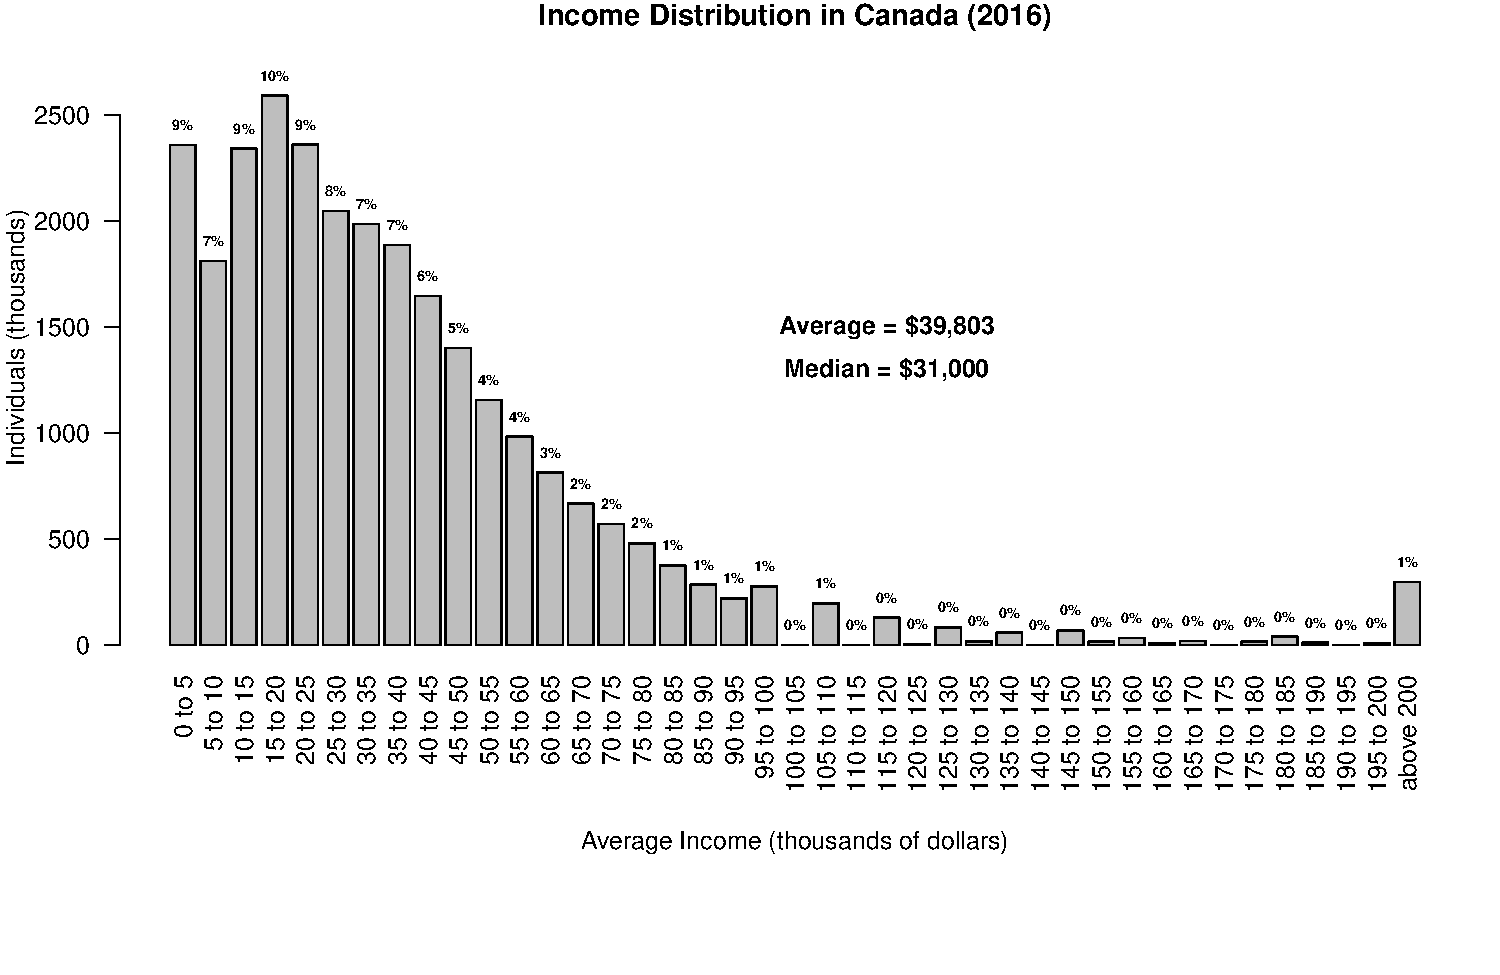
\includegraphics[width=0.8\linewidth]{week7/week7-dist1-1} 

\end{knitrout}
\end{center}
We can see from the histogram that there is a concentration of
individuals in the bottom of the distribution (low income groups): The
distribution is skewed to the right with a peak for the income group
\$200,000 and above. The histogram shows clearly that income
inequality is present in Canada. 

\subsubsection*{Distribution of Income Across Households}

The above graph is the distribution of income at the individual level
for the working age population. Some of the low income individuals are
students working few hours per year and others are members of high
income families who are voluntarily out of the labour force. For that
reason, it may be more appropriate instead to look at the household
income distribution because an household income includes income of all
members of the household. That information is available on the
Statistics Canada website, in table 11-10-0237-01
\citep*{distribution}. The following graph shows the distribution of
household after-tax income in 2018. You obtain the information by
selecting After-tax income in the \textbf{Income concept} tab,
Economic families and persons not in an economic families in the
\textbf{Economic family type} tab and all income groups in the
\textbf{Statistics} tab of the table. The number on the top of each
bar is the proportion of households that belong to that particular
income group.
\begin{center}
\begin{knitrout}\footnotesize
\definecolor{shadecolor}{rgb}{0.969, 0.969, 0.969}\color{fgcolor}
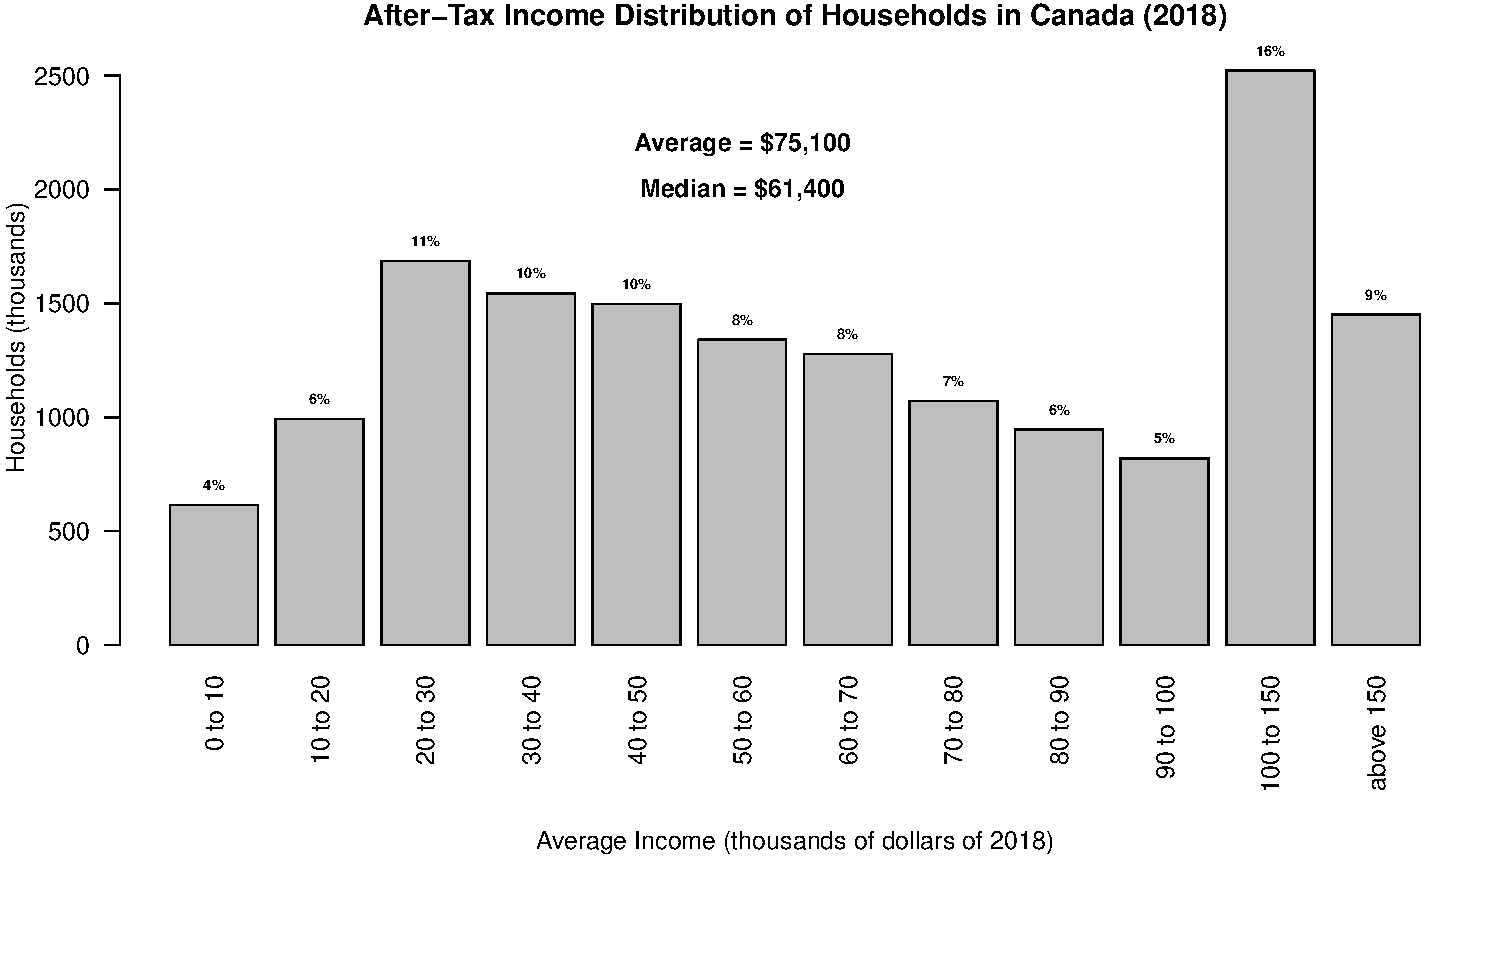
\includegraphics[width=0.8\linewidth]{week7/week7-dist2-1} 

\end{knitrout}
\end{center}
We can see that the number of income groups is smaller: we have only
12 income groups while we had 41 groups on the individual based income
distribution. This is the best we can do using the formatted tables
from Statistics Canada. We do, however, observe the same shape: a
concentrated number of households at the bottom of the distribution
(41\% of households have income less than \$50,000) and a peak at the
top (27\% of households have income greater than
\$100,000). Therefore, the income distribution is also unequal at the
household level. Notice that this histogram also provides an imperfect
picture of the income distribution because households are not of the
same sizes. 



\subsection{Measuring Inequality: Average Versus Median Income}

On the two graphs we also see that average income at the individual
and household levels are respectively \$39,803 and
\$75,100, and the medians are respectively \$31,000 and
\$61,400. 

\subsubsection*{Median}

The median is the value that separates the population in two equal
groups. Therefore, individual incomes are higher than \$31,000
for 50\% of the population and household incomes are higher than
\$61,400 for 50\% of households. The averages are higher than
the medians because many individuals and households have very high
income compared with the average Canadians. The average is much more
influenced by the right tail of the distribution (high income groups)
than the median. To understand why, suppose Canada is composed of 4
individuals. The following table shows the income of all individuals
for 2015 and 2020 with the average and median income for each year.
\begin{center}
\begin{tabular}{lcccc||cc}
Year &Individual 1&Individual 2&Individual 3 & Individual 4 & Average&
Median\\\hline 2015 Income & \$100 & \$200 & \$202 & \$302 & \$201 &
\$201\\ 2020 Income & \$100 & \$200 & \$202 & \$400 & \$225.5 & \$201
\end{tabular}
\end{center}
In 2015, the median is \$201 because the income is greater than \$201
for 50\% of the population (individuals 3 and 4) and it is less than
\$201 for 50\% of the population (individuals 1 and 2), and the
average is also \$201: (\$100+\$200+\$202+\$302)/4=\$201. From 2015 to
2020, the income of the fourth individual has increased to \$400 while
all other incomes have remained constant. Therefore, the median in
2020 is the same as in 2015 because we still have 50\% of incomes on
either side of \$201. However, the average has increased to \$225.5
and is higher than the median:
(\$100+\$200+\$202+\$400)/4=\$225.5. Therefore, when we only increase
the income of the richest individuals, the average increases and
median remains unaffected. It is therefore a sign that the allocation
is becoming more unequal when the gap between the average and the
median is increasing.

\subsubsection*{The Evolution of Average and Median Income in Canada}

The average and median incomes in dollars of 2018 from 1976 to 2018
are available from the same Statistics Canada table by selecting
Average Income and Median Income from the \textbf{Statistics} tab. The
following graph plots the two series (the solid black line is the
average income and the dashed blue line is the median income
series). First, we see that both statistics decreased slightly on
average between 1976 and the mid '90s and increased from the mid '90s
to 2018. Second, the gap between the average and the median increased
over the period, going from 6.2 to
13.7 thousand dollars of 2018
(see the gaps represented by the arrows). This is a sign that income
inequality has increased over this period.



\begin{center}
\begin{knitrout}\footnotesize
\definecolor{shadecolor}{rgb}{0.969, 0.969, 0.969}\color{fgcolor}
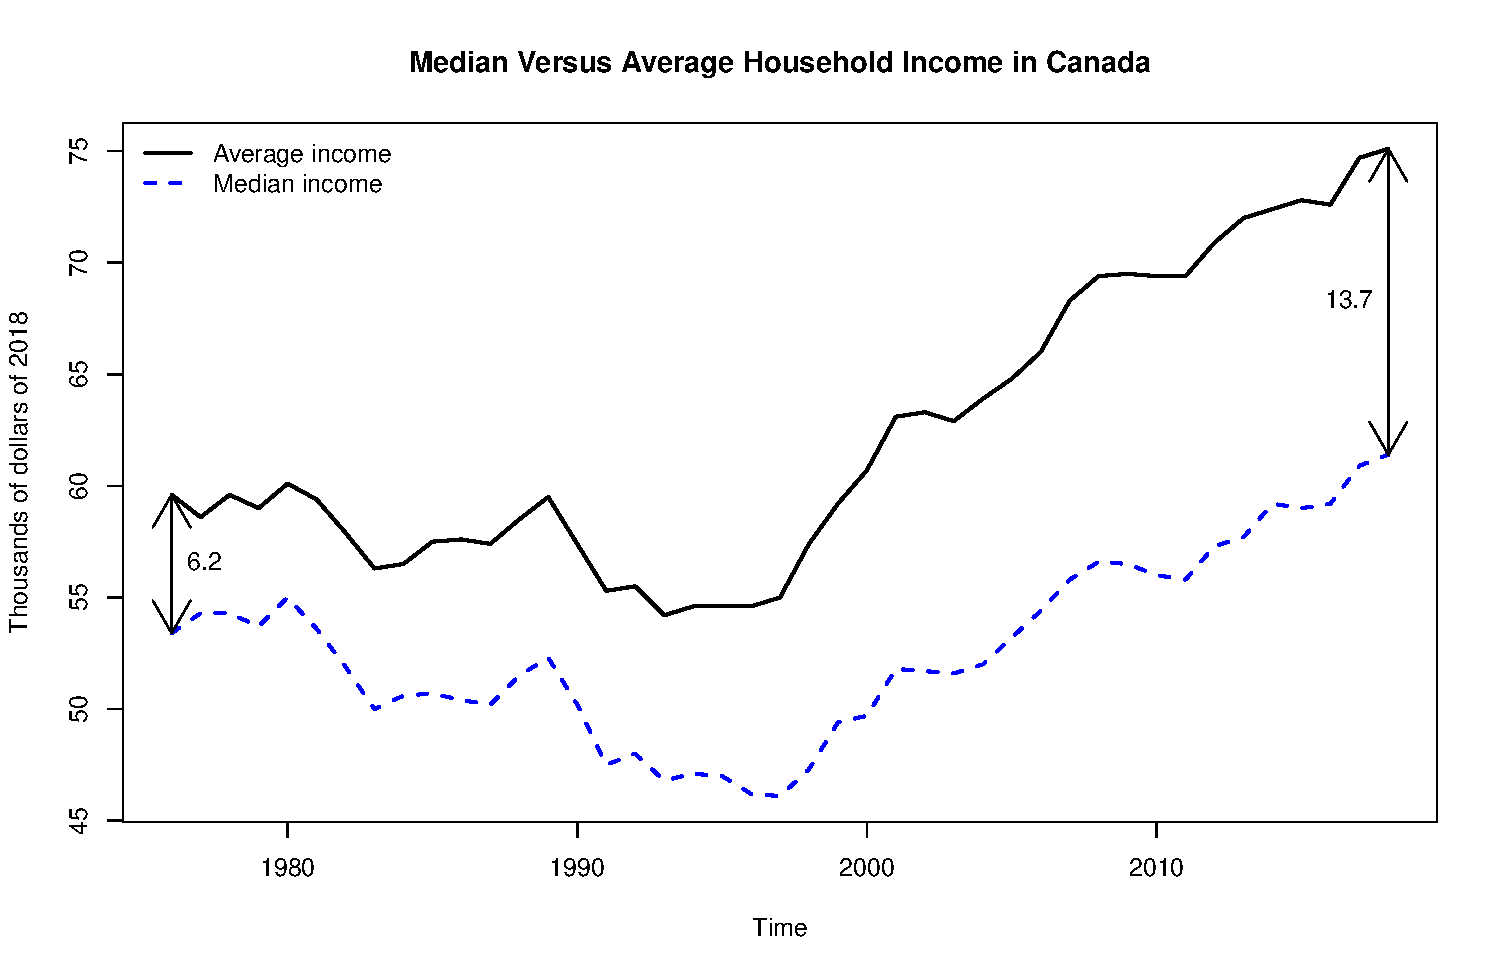
\includegraphics[width=0.8\linewidth]{week7/week7-dist5-1} 

\end{knitrout}
\end{center}


\subsection{Measuring Inequality: The Gini Coefficient}

Comparing inequality across regions or countries using histograms is
difficult because it is not evident what we should be comparing. The
purpose of the Gini coefficient is to provide one number that
characterizes the level of inequality. The coefficient can be used to
compare regions and periods.

\subsubsection*{The Lorenz Curve}

The Lorenz Curve is a visualization tool to analyze income
inequality. To plot the curve, we need the share of total income by
quintile. The following table is the same one use in previous section. 
\begin{center}
\resizebox{0.9\linewidth}{!}{  
% latex table generated in R 3.6.3 by xtable 1.8-4 package
% Fri Apr 24 16:50:15 2020
\begin{tabular}{lcc}
  \multicolumn{3}{c}{\textbf{Average Income by Quintile in 2018}} \\
 \hline
 & Average Household Income (dollars) & Share of Total Household Income (percent) \\ 
  \hline
First Income Quintile & 23,537 & 5.90 \\ 
  Second Income Quintile & 49,137 & 12.40 \\ 
  Third Income Quintile & 69,943 & 17.60 \\ 
  Fourth Income Quintile & 91,798 & 23.10 \\ 
  Fifth Income Quintile & 162,231 & 40.90 \\ 
   \hline
\end{tabular}

} 
\end{center} 

We first need the cumulative share of household income. The cumulative
share of income is the share of income of the first quintile (the 20\%
poorest), the first two quintiles (the 40\% poorest), the first three
(the 60\% poorest) and so on. It is the cumulative sum of the second
column and is represented in the following table:
\begin{center} 
\resizebox{0.5\linewidth}{!}{
% latex table generated in R 3.6.3 by xtable 1.8-4 package
% Fri Apr 24 16:50:15 2020
\begin{tabular}{lc}
  \multicolumn{2}{c}{\textbf{Cumulative Income Share in Canada in 2018}} \\
 \hline
 & Cumulative Income Share (percent) \\ 
  \hline
The bottom 20\% & 5.90 \\ 
  The bottom 40\% & 18.30 \\ 
  The bottom 60\% & 35.90 \\ 
  The bottom 80\% & 59.00 \\ 
  The bottom 100\% & 99.90 \\ 
   \hline
\end{tabular}

}
\end{center}
The first value is 5.9, the second is
5.9+12.4=18.3, the third is
5.9+12.4+17.6=35.9
and so on. The last value is not exactly 100\% because of rounding
errors. The Lorenz curve, plots the values of the second column as a
function of the values in the first column. The chart also includes the
perfect equality curve. Income is perfectly equal if the share of
total income of the bottom 20\% of the distribution is 20\%, it is
40\% for the bottom 40\% and so on. 

The following graph shows the Lorenz curve for Canada in 2018 (the
blue line with round markers) and for the United States in 2009 (the
red line with triangular markers) using the data from the module
readings. The solid black line is the perfect equality line and the
coordinates are specified for Canada only for clarity. The further
away the curve is from the perfect equality line, the more unequal is
the income allocation. Therefore, we can conclude that the 2009
allocation in the USA is more unequal than the 2018 allocation in
Canada. 
\begin{center}
\begin{knitrout}\footnotesize
\definecolor{shadecolor}{rgb}{0.969, 0.969, 0.969}\color{fgcolor}
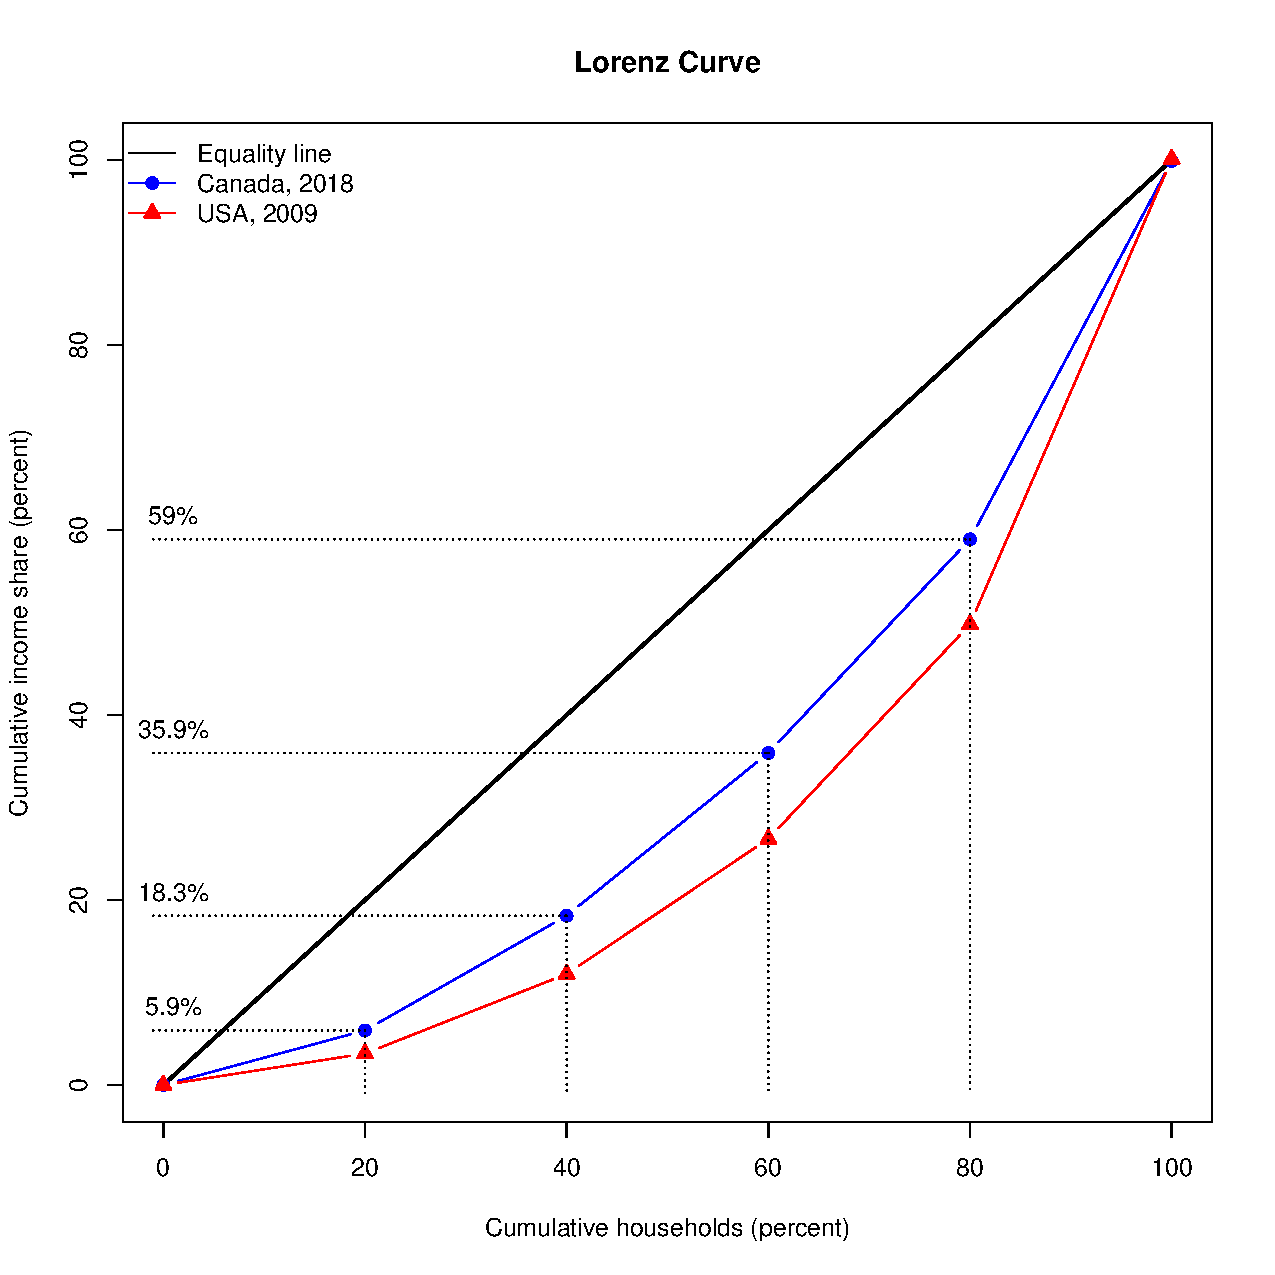
\includegraphics[width=0.6\linewidth]{week7/week7-dist7-1} 

\end{knitrout}
\end{center}



\subsubsection*{The Gini Coefficient}

The Gini coefficient is a measure based on the Lorenz curve. It is the
area between the perfect equality line and the Lorenz curve divided by
the area below the equality line. Since the equality line and the axes
form a right triangle with a base of 1 (100\%) and a height of 1
(100\%), the area under the equality line is 0.5. Therefore the Gini
coefficient is twice the area between the equality line and the Lorenz
curve. Therefore, the coefficient is equal to 0 if the Lorenz curve is
equal to the equality line and it increases as the allocation becomes
more unequal. Let $h_i=(i/5-s_i)$, for $i=1,2,3,4$, be the distance
between the equality line and the Lorenz curve at 20\%, 40\%, 60\% and
80\% respectively, where $s_i$ is the cumulative income share of
quintiles 1 to i. Then, the Gini coefficient is:
\[
\mathcolorbox{
\mathrm{Gini} = 0.40 \times (h_1+h_2+h_3+h_4) = 0.8-0.4\times(s_1+s_2+s_3+s_4)}
\]
Using this formula, the maximum Gini coefficient is reached when all
shares are equal to zero which gives a coefficient of 0.8. To have a
coefficient of 1 in the most unequal allocation, we need to divide the
population in more than 5 groups.

\begin{background}
We can derive the Gini coefficient formula using basic geometry. If we
look at the chart between two points, we get the following:
\begin{center}
\begin{knitrout}\footnotesize
\definecolor{shadecolor}{rgb}{0.969, 0.969, 0.969}\color{fgcolor}
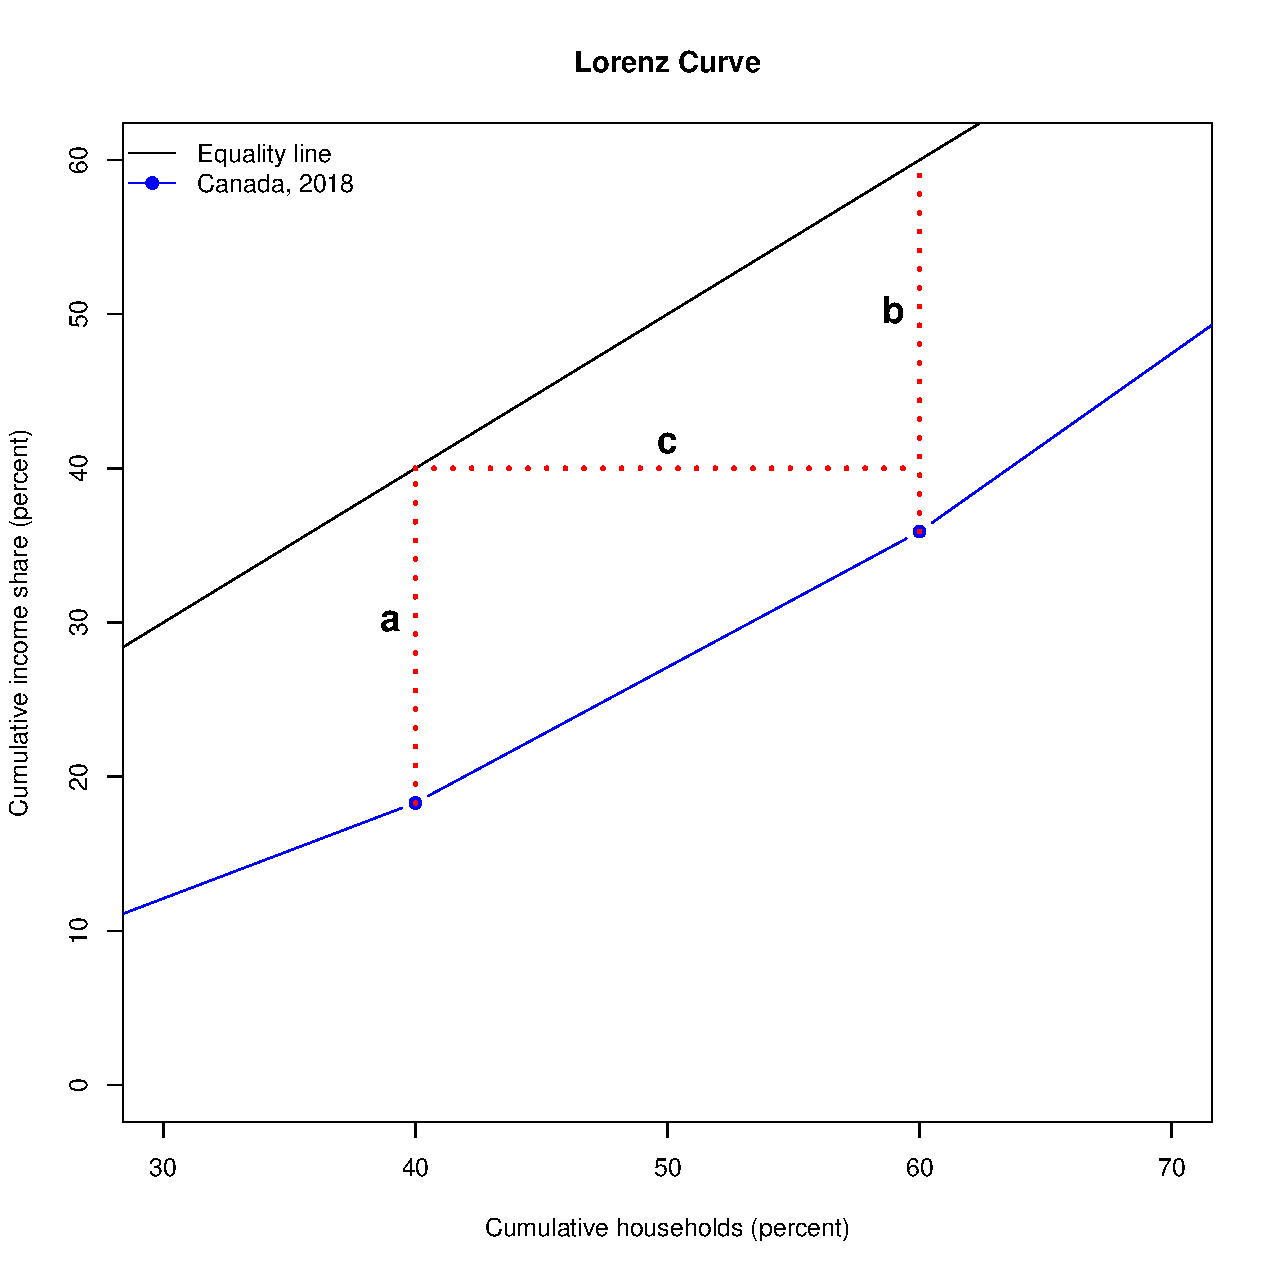
\includegraphics[width=0.4\linewidth]{week7/week7-dist10-1} 

\end{knitrout}
\end{center}
The area between the Lorenz curve and the equality curve between the
two points is the area of the trapezoid with bases a and b and height
c. The formula for the area of a trapezoid is
(a+b)$\times$c/2. According to our above definition a and b are
respectively $h_2$ and $h_3$ and c is equal to 0.20 (20\%). To compute
the Gini coefficients we need to add the areas between each points and
multiply the result by 2. In other words, we need to add the areas A
to E in the following graph:
\begin{center}
\begin{knitrout}\footnotesize
\definecolor{shadecolor}{rgb}{0.969, 0.969, 0.969}\color{fgcolor}
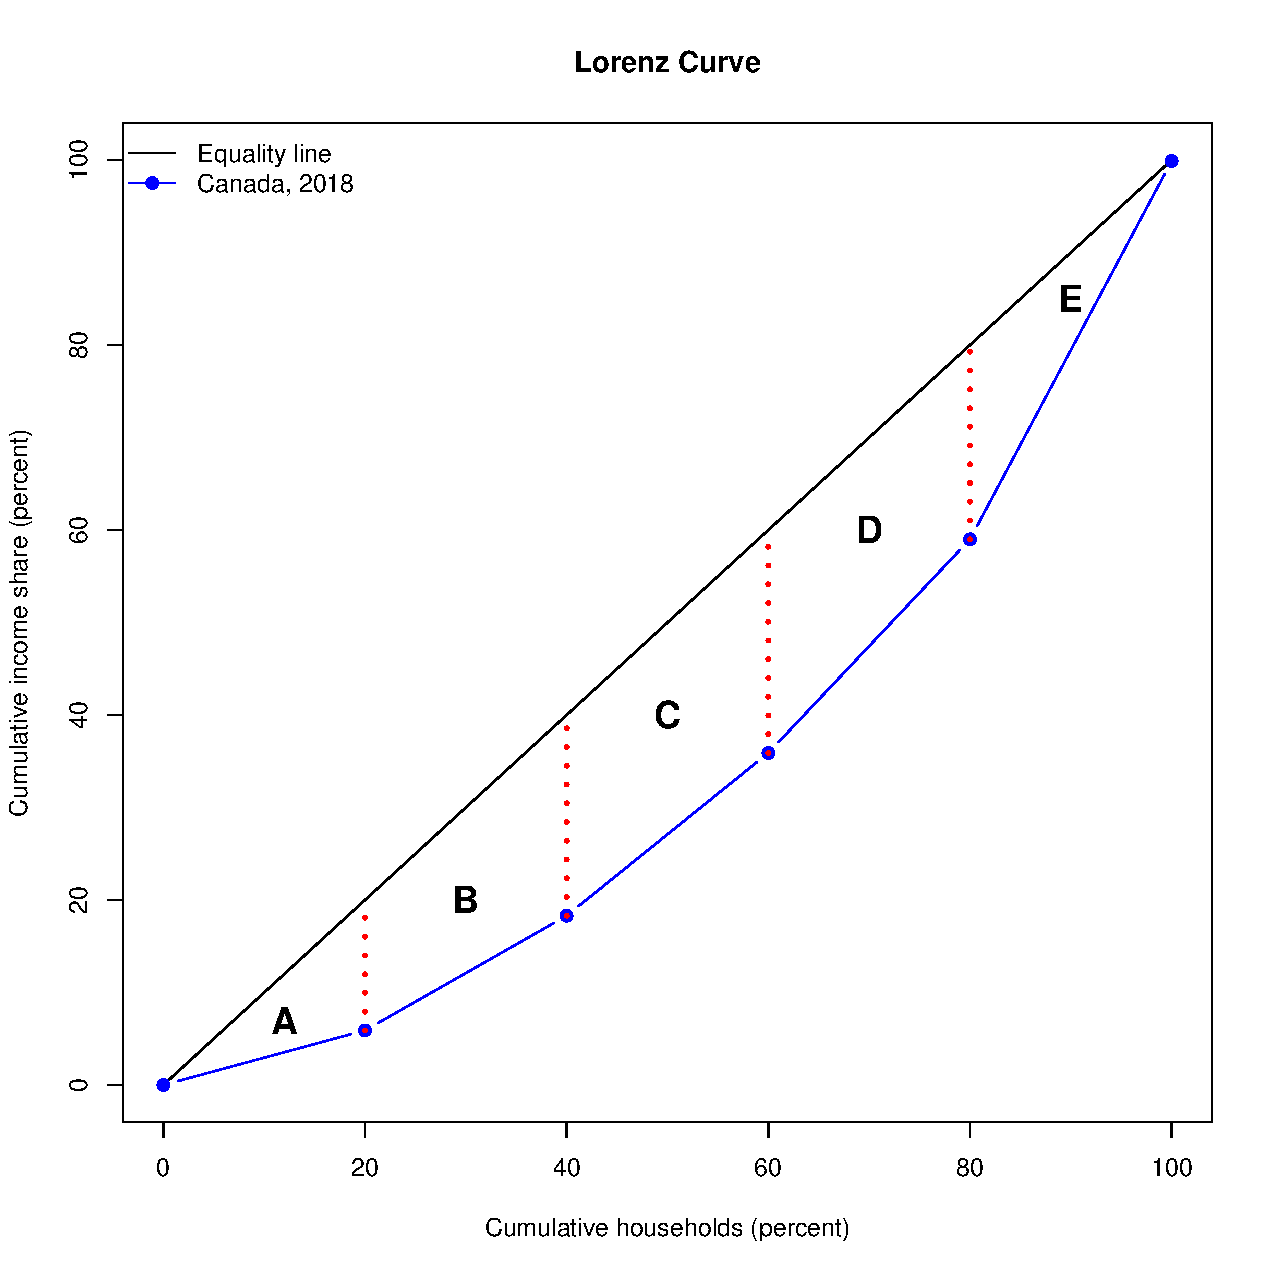
\includegraphics[width=0.4\linewidth]{week7/week7-dist11-1} 

\end{knitrout}
\end{center}
For A and E, we use the same formula with a=0 for A and b=0 for E. The
Gini coefficient is therefore: 
\footnotesize
\begin{eqnarray*}
  \mathrm{Gini} &=& 2\times \left(\frac{0.20\times h_1}{2} +
   \frac{0.20\times (h_1+h_2)}{2}+
   \frac{0.20\times (h_2+h_3)}{2}+
   \frac{0.20\times (h_3+h_4)}{2} +
   \frac{0.20\times h_4}{2}\right)\\
         & = & 0.40 \times \left(h_1+h_2+h_3+h_4\right)
\end{eqnarray*}
\normalsize In general, if we split the population in n equal groups,
we have n-1 $h_i=(i/n-s_i)$, where $s_i$ is the cumulative income
share of groups 1 to i, and c=1/n in the trapezoid area formula. Using
the same logic, we can compute the Gini coefficient using the
following formula:
\[
\mathrm{Gini} = \frac{2}{n}\sum_{i=1}^{n-1} h_i
\]
Replacing $h_i$ by its value, we get:
\[
\mathrm{Gini} = \frac{2}{n}\sum_{i=1}^{n-1} (i/n-s_i) = 
\frac{n-1}{n} - \frac{2}{n}\sum_{i=1}^{n-1} s_i\,,
\]
where we used the fact that $1+2+3+4+\cdots + (n-1)=n(n-1)/2$.  Notice
that if we divide the population in quintiles, n=5 and we get the same
formula. The maximum is reached when all $s_i$ are equal to zero which
implies a Gini coefficient of (n-1)/n. Therefore it approaches 1 when n
gets very large, which implies a very large population in which total
income is allocated to only one individual.
\end{background}

\subsubsection*{Gini Coefficient in Canada and the United States}

The following table shows the 2018 cumulative income share for Canada
and the 2009 cumulative income share for the United States (see the
module readings). 
\begin{center} 
\resizebox{0.5\linewidth}{!}{
% latex table generated in R 3.6.3 by xtable 1.8-4 package
% Fri Apr 24 16:50:15 2020
\begin{tabular}{lcc}
  \multicolumn{3}{c}{\textbf{Cumulative Income Share}} \\
 \hline
 & Canada, 2018 (percent) & USA, 2009 (percent) \\ 
  \hline
The bottom 20\% & 5.90 & 3.40 \\ 
  The bottom 40\% & 18.30 & 12.00 \\ 
  The bottom 60\% & 35.90 & 26.60 \\ 
  The bottom 80\% & 59.00 & 49.80 \\ 
  The bottom 100\% & 99.90 & 100.10 \\ 
   \hline
\end{tabular}

}
\end{center}
Once more, numbers from the last row should be equal to 100. The
differences are explained by rounding error. Using the formula with
shares, the Gini coefficients for Canada and the United States are
respectively:
\[
\mbox{Gini for Canada} = 0.8 - 0.4\times
(0.059+0.183+0.359+0.59) = 0.3236
\]
and
\[
\mbox{Gini for the USA} = 0.8 - 0.4\times
(0.034+0.12+0.266+0.498) = 0.4328\,.
\]
According to the Gini coefficients, the allocation of income is less
equal in the United States compared with Canada because the Gini
coefficient is higher for the US.



\subsubsection*{The Limit of the Gini Coefficient}

As we may expect, the Gini coefficient is an imperfect measure of
income inequality. We cannot expect one number to provide a complete
picture of income allocation. In fact, if the sum of the income shares
remains the same the coefficient is unchanged. If we consider the 2018
distribution in Canada:
\begin{center}
\resizebox{0.9\linewidth}{!}{  
% latex table generated in R 3.6.3 by xtable 1.8-4 package
% Fri Apr 24 16:50:15 2020
\begin{tabular}{lcc}
  \multicolumn{3}{c}{\textbf{Income share in 2018}} \\
 \hline
 & Share of Total Household Income (percent) & Cumulative Income Share (percent) \\ 
  \hline
First Income Quintile & 5.90 & 5.90 \\ 
  Second Income Quintile & 12.40 & 18.30 \\ 
  Third Income Quintile & 17.60 & 35.90 \\ 
  Fourth Income Quintile & 23.10 & 59.00 \\ 
  Fifth Income Quintile & 40.90 & 99.90 \\ 
   \hline
\end{tabular}

} 
\end{center} 
Suppose that income is shifted from the first to the second quintile
(the poor get poorer) and from the fourth to the fifth quintile (the
rich get richer) as follows:
\begin{center}
\resizebox{0.9\linewidth}{!}{  
% latex table generated in R 3.6.3 by xtable 1.8-4 package
% Fri Apr 24 16:50:15 2020
\begin{tabular}{lcc}
  \multicolumn{3}{c}{\textbf{Alternative Income share}} \\
 \hline
 & Share of Total Household Income (percent) & Cumulative Income Share (percent) \\ 
  \hline
First Income Quintile & 2.90 & 2.90 \\ 
  Second Income Quintile & 15.40 & 18.30 \\ 
  Third Income Quintile & 17.60 & 35.90 \\ 
  Fourth Income Quintile & 15.10 & 51.00 \\ 
  Fifth Income Quintile & 48.90 & 99.90 \\ 
   \hline
\end{tabular}

} 
\end{center}
Clearly, the allocation is more unequal, but the Gini coefficient is
the same:
\[
\mbox{Gini} = 0.8 - 0.4\times
(0.034+0.12+0.266+0.498) = 0.4328\,.
\]
Therefore, we have to keep in mind that the Gini coefficient is one
tool to compare inequalities, but it does not tell us everything about
income distribution. For a complete picture, we need to dig deeper.

\subsubsection*{Gini Coefficient in General} 

The Gini coefficient is not in general based on quintiles. Instead,
the population is divided in many groups. It is even possible to
compute the Gini coefficient using individual incomes. In that case,
each individual is a group. When we divide the population into n equal
groups. the formula is:
\[\mathcolorbox{
\mathrm{Gini} = \frac{2}{n}\sum_{i=1}^{n-1} (i/n+s_i) = 
\frac{n-1}{n} - \frac{2}{n}\sum_{i=1}^{n-1} s_i}\,,
\]
where $n$ is the number of groups (n=5 when the population is divided
in quintiles) sorted by income and $s_i$ is the income share of the
groups 1 to i. If we use the same data that produced the income
distribution at the individual level earlier in this module, we get a
Gini coefficient of 0.45. It reflects what we saw that the allocation
is much more unequal at the individual level. The following graph
compares the Lorenz curves at the household (red with round markers)
and individual (dashed blue line) levels. We can see that the more
groups we have the smoother is the Lorenz curve. It is also clear that
there is more inequality at the individual level.
\begin{center}
\begin{knitrout}\footnotesize
\definecolor{shadecolor}{rgb}{0.969, 0.969, 0.969}\color{fgcolor}
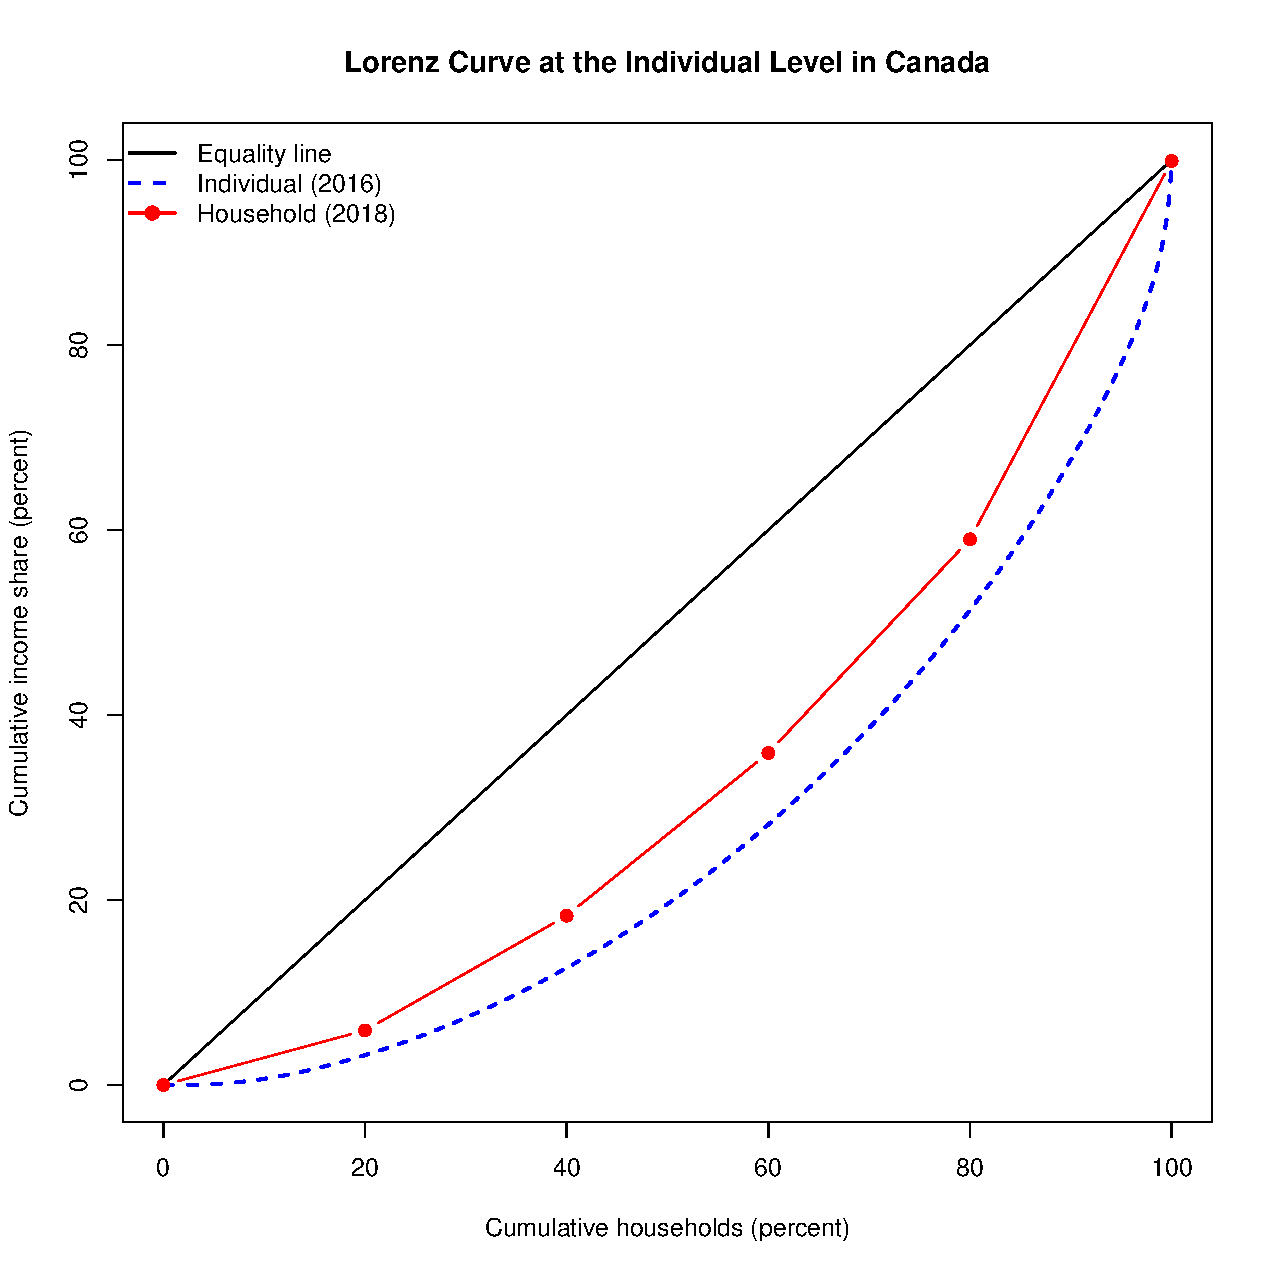
\includegraphics[width=0.5\linewidth]{week7/week7-dist12-1} 

\end{knitrout}
\end{center}

\subsubsection*{The Evolution of the Gini Coefficient in Canada}

Statistics Canada publishes an annual series of the Gini coefficient
that starts in 1976 \citep*{gini}. We discussed in a previous section
that the histogram of household incomes can be misleading because it
does not take into account the size of the households. The Gini
coefficient computed by Statistics Canada is based in household income
adjusted for family size. The following is the Gini coefficient based
on the adjusted after-tax income (it is income from all sources
including government transfer less income tax). First, the coefficient
was constant on average from 1976 to the end of the '80s, then
increased from the early '90s to the early 2000s (an increase in
income inequality) and start decreasing onward. We also notice that
the business cycle affects inequality. For example, we can see the
increase of the coefficient during the recessions of 1982 and 1990.

\begin{center}
\begin{knitrout}\footnotesize
\definecolor{shadecolor}{rgb}{0.969, 0.969, 0.969}\color{fgcolor}
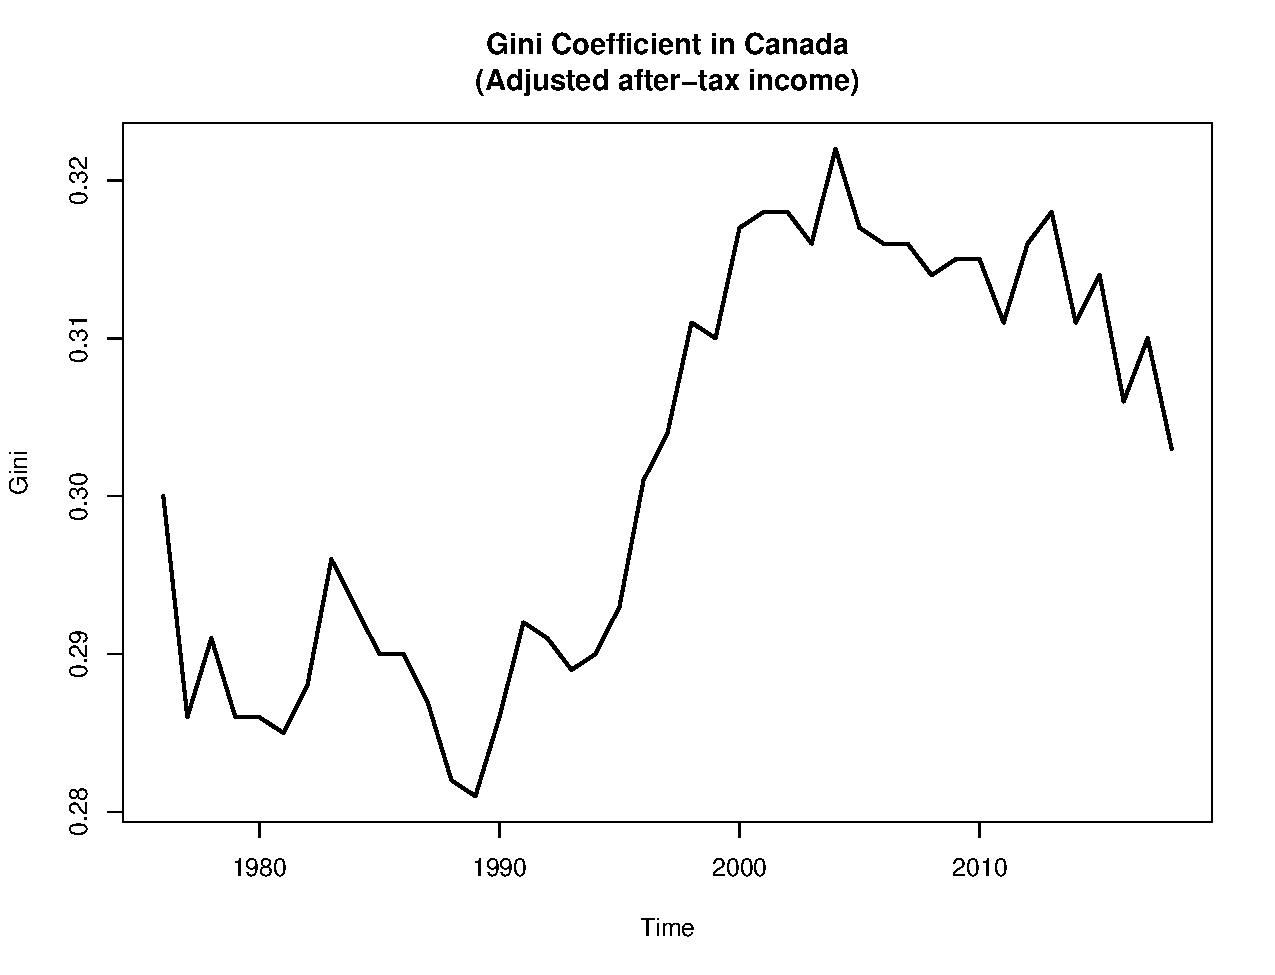
\includegraphics[width=0.5\linewidth]{week7/week7-dist13-1} 

\end{knitrout}
\end{center}

The following graph compares the Gini coefficient of four
provinces. The Ontario province (dot-dashed blue line) is where
inequality has increased the most over the period and at the end of
2018, the provinces with least income inequality was New Brunswick
(dashed red) and Quebec (dotted green).

\begin{center}
\begin{knitrout}\footnotesize
\definecolor{shadecolor}{rgb}{0.969, 0.969, 0.969}\color{fgcolor}
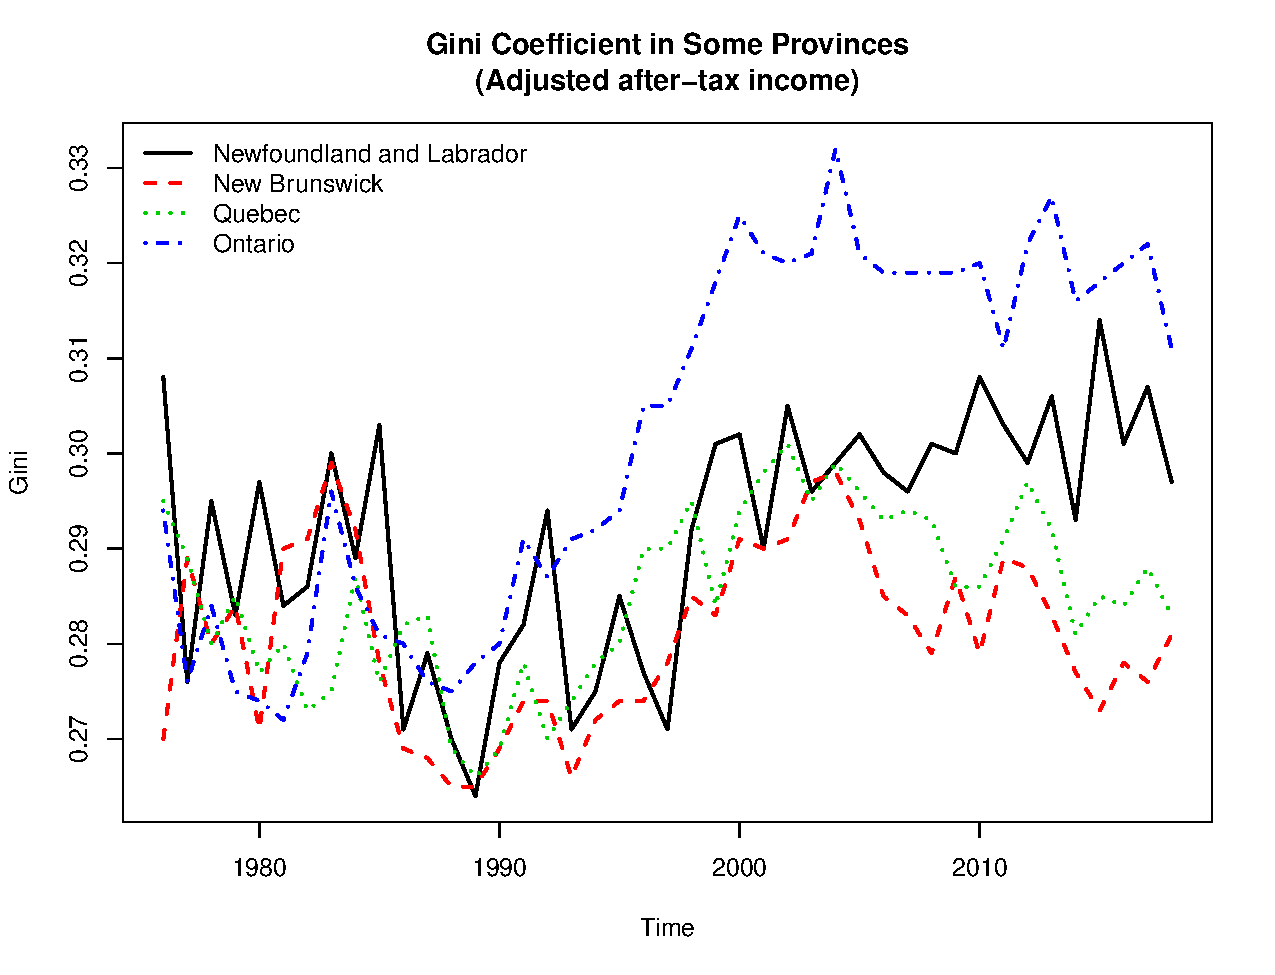
\includegraphics[width=0.5\linewidth]{week7/week7-dist14-1} 

\end{knitrout}
\end{center}



\subsubsection*{Comparing the Gini Coefficient Across Countries}

We can compare inequality across countries using the Gini coefficient,
but it has to come from the same source. Coefficients from different
sources may be computed differently. For example, the type of income
used to calculate the coefficient may differ. The OECD published
annual time series of the Gini coefficient for several countries
\citep*{oecd-gini}. It is based on after-tax and after-transfer
income. You can access the bar chart to compare the most recent
coefficient across countries at
\href{https://data.oecd.org/chart/5VBS}{https://data.oecd.org/chart/5VBS}
and the times series at
\href{https://data.oecd.org/chart/5VBV}{https://data.oecd.org/chart/5VBV}. The
links offer interactive graphs that allow to navigate through
different countries. You can also download the data and produce your
own graphs. The following is the bar chart of the Gini coefficient in
2015 for several countries. According to the Gini coefficient, Canada
is in the middle of the shown countries in terms of inequality and the
United States is among the most unequal countries. Slovakia is the
most equal and South Africa is the most unequal country.

\begin{center}
\begin{knitrout}\footnotesize
\definecolor{shadecolor}{rgb}{0.969, 0.969, 0.969}\color{fgcolor}
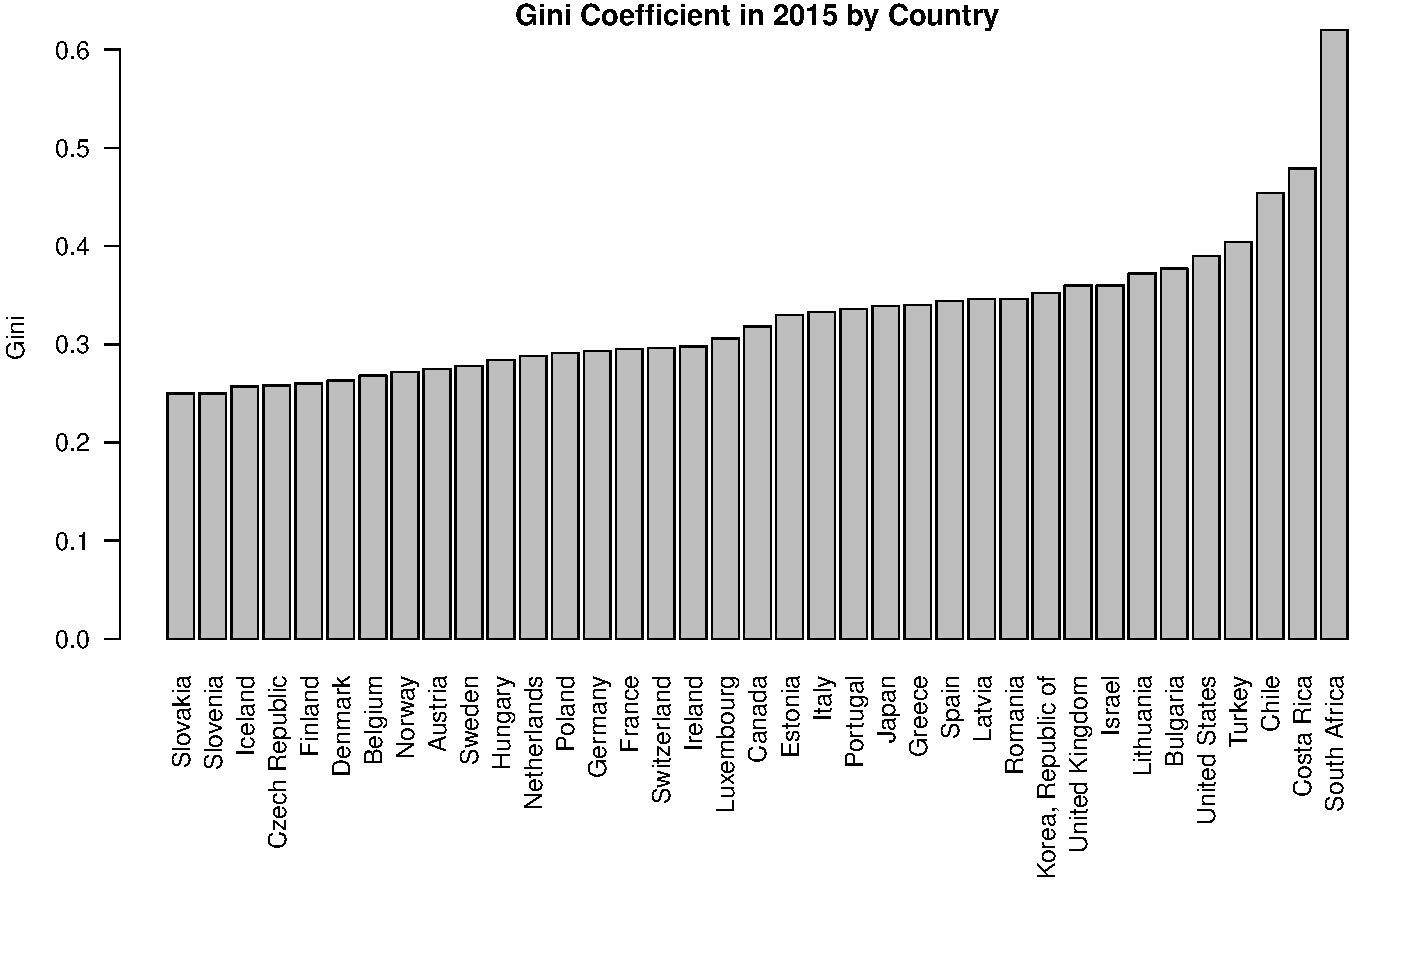
\includegraphics[width=0.6\linewidth]{week7/week7-dist15-1} 

\end{knitrout}
\end{center}

\subsubsection*{Exercises: Measuring the Gini Coefficient}


\begin{enumerate}
\item Consider the following table  
\begin{center}  
\resizebox{0.5\linewidth}{!}{    
% latex table generated in R 3.6.3 by xtable 1.8-4 package
% Fri Apr 24 16:50:17 2020
\begin{tabular}{lc}
  \hline
 & Average Income (dollars) \\ 
  \hline
First Income Quintile & 342 \\ 
  Second Income Quintile & 642 \\ 
  Third Income Quintile & 844 \\ 
  Fourth Income Quintile & 990 \\ 
  Fifth Income Quintile & 1,053 \\ 
   \hline
\end{tabular}

}
\end{center}  
Compute the Gini coefficient.
\item Consider the following table  
\begin{center}    
\resizebox{0.5\linewidth}{!}{      
% latex table generated in R 3.6.3 by xtable 1.8-4 package
% Fri Apr 24 16:50:17 2020
\begin{tabular}{lc}
  \hline
 & Average Income (dollars) \\ 
  \hline
First Income Decile & 114 \\ 
  Second Income Decile & 288 \\ 
  Third Income Decile & 605 \\ 
  Fourth Income Decile & 621 \\ 
  Fifth Income Decile & 1,012 \\ 
  Sixth Income Decile & 1,023 \\ 
  Seventh Income Decile & 1,101 \\ 
  Eighth Income Decile & 1,434 \\ 
  Nineth Income Decile & 1,925 \\ 
  Tenth Income Decile & 1,934 \\ 
   \hline
\end{tabular}

}
\end{center}  
Compute the Gini coefficient.
\end{enumerate}

\subsubsection*{Solution}
\begin{enumerate}
\item First, we compute the income share. It is the average income of
  each quintile divided the the sum of the average incomes. For example, the income share of the first quintile is:
\[
S_1 = \frac{342}{
  342+642+844+990+1,053}=
8.83\%
\]
In the second quintile, it is equal to :
\[
S_2 = \frac{642}{
  342+642+844+990+1,053}=
16.58\%
\]
Then, we compute the cumulative income share: The first is
8.83\%, the second is
(8.83\%+16.58\%),
and so on. The following table shows the shares and cumulative shares
(numbers were rounded at the end)
\begin{center}  
\resizebox{0.9\linewidth}{!}{    
% latex table generated in R 3.6.3 by xtable 1.8-4 package
% Fri Apr 24 16:50:17 2020
\begin{tabular}{lccc}
  \hline
 & Average Income (dollars) & Income share (percent) & Cumulative shares (percent) \\ 
  \hline
First Income Quintile & 342 & 8.83 & 8.83 \\ 
  Second Income Quintile & 642 & 16.58 & 25.42 \\ 
  Third Income Quintile & 844 & 21.80 & 47.22 \\ 
  Fourth Income Quintile & 990 & 25.57 & 72.80 \\ 
  Fifth Income Quintile & 1,053 & 27.20 & 100.00 \\ 
   \hline
\end{tabular}

}
\end{center}  
Then, we use the formula:
\[
\mathrm{Gini} = 0.8-0.4\times(s_1+s_2+s_3+s_4)\,,
\]
where $s_i$ are the comulative shares. The coefficient is therefore:
\[
\mathrm{Gini} = 0.8-0.4\times(0.0883+0.2542+0.4722+0.728) = 0.18
\]
\item First, we compute the income share. It is the average income of
  each decile divided the the sum of the average incomes. For example,
  the income share of the first decile is:
\footnotesize  
\[
S_1 = \frac{114}{
  114+288+605+621+1,012+1,023+1,101+1,434+1,925+1,934}=
1.13\%
\]
\normalsize
In the second decile, it is equal to :
\footnotesize
\[
S_2 = \frac{288}{
  114+288+605+621+1,012+1,023+1,101+1,434+1,925+1,934}=
2.86\%
\]
\normalsize
Then, we compute the cumulative income share: The first is
1.13\%, the second is
(1.13\%+2.86\%),
and so on. The following table shows the shares and cumulative shares
(numbers were rounded at the end)
\begin{center}  
\resizebox{0.9\linewidth}{!}{    
% latex table generated in R 3.6.3 by xtable 1.8-4 package
% Fri Apr 24 16:50:17 2020
\begin{tabular}{lccc}
  \hline
 & Average Income (dollars) & Income share (percent) & Cumulative shares (percent) \\ 
  \hline
First Income Decile & 114 & 1.13 & 1.13 \\ 
  Second Income Decile & 288 & 2.86 & 4.00 \\ 
  Third Income Decile & 605 & 6.02 & 10.01 \\ 
  Fourth Income Decile & 621 & 6.17 & 16.19 \\ 
  Fifth Income Decile & 1,012 & 10.06 & 26.25 \\ 
  Sixth Income Decile & 1,023 & 10.17 & 36.42 \\ 
  Seventh Income Decile & 1,101 & 10.95 & 47.37 \\ 
  Eighth Income Decile & 1,434 & 14.26 & 61.63 \\ 
  Nineth Income Decile & 1,925 & 19.14 & 80.77 \\ 
  Tenth Income Decile & 1,934 & 19.23 & 100.00 \\ 
   \hline
\end{tabular}

}
\end{center}  
Then, we use the formula:
\[
\mathrm{Gini} = \frac{n-1}{n}-\frac{2}{n}\times(s_1+s_2+\cdots+s_{9})\,,
\]
where $s_i$ are the comulative shares and $n=10$. The coefficient is
therefore:
\footnotesize
\[
\mathrm{Gini} = 0.9-0.2\times(0.0113+0.04+0.1001+0.1619+0.2625+0.3642+0.4737+0.6163+0.8077) = 0.33
\]
\normalsize
\end{enumerate}  


  
\subsection{Measure of Poverty}
Income inequality is particularly problematic when it implies that a
large proportion of the population is in a state of poverty. How do we
define poverty and how do we measure it is the topic of this
section. An household is considered poor if its income falls below the
poverty line. Two of the measures used by Statistics Canada are the
market basket measure and the low income measure. In this section, we
use the Statistics Canada table 11-10-0135-01 \citep*{poverty}

\subsubsection*{The Market Basket Measure}

The Statistics Canada definition of the market basket measure (MBM) is
(Footnote 7 of the table):

\say{The Market Basket Measure (MBM) is based on the cost of a
  specific basket of goods and services representing a modest, basic
  standard of living. It includes the costs of food, clothing,
  shelter, transportation and other items for a reference
  family. These costs are compared to the disposable income of
  families to determine whether or not they fall below the poverty
  line}

Therefore, an household is considered to be below the poverty line if
they cannot afford the ``modest and basic standard of living''
determined by the basket.  The table includes the proportion of
persons that are below that poverty line by characteristics (sex, age,
etc.) starting in 2006. The following bar chart shows the proportions
for some groups in 2018. We can see that 24.6\%
of the persons who do not live in an economic families (a group of two
and more persons living in the same dwelling) are below that poverty
line. It is clearly the group of persons who is the most affected by
poverty. Also, the group with the smallest proportion of persons below
the poverty line is the 65 years and over, followed by the persons
living in an economic families.

\begin{center}
\begin{knitrout}\footnotesize
\definecolor{shadecolor}{rgb}{0.969, 0.969, 0.969}\color{fgcolor}
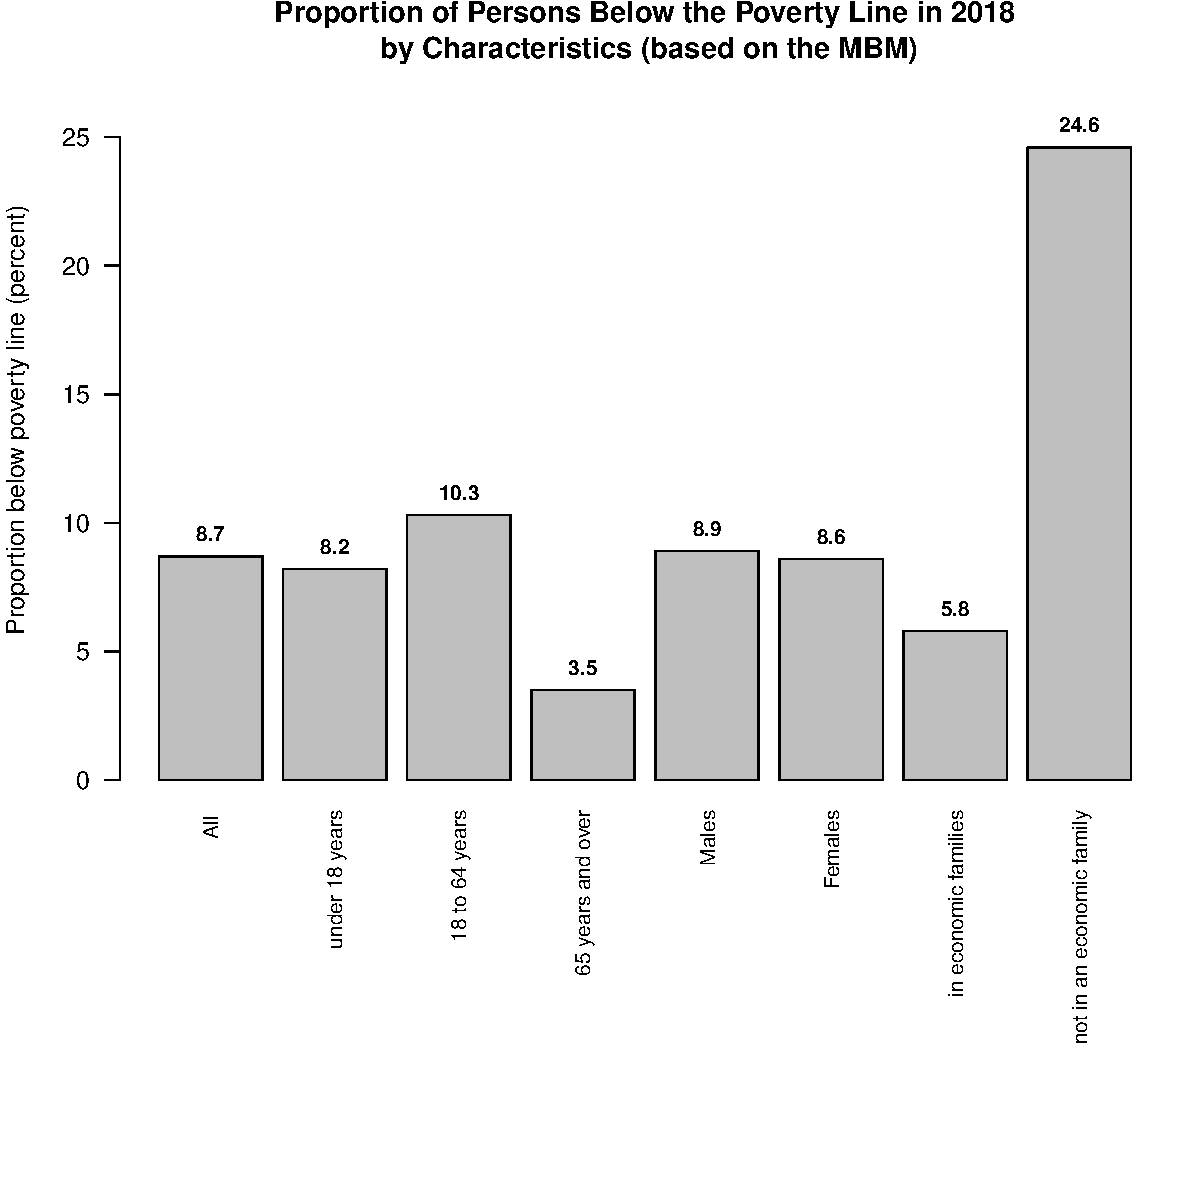
\includegraphics[width=0.6\linewidth]{week7/week7-poverty1-1} 

\end{knitrout}
\end{center}



\subsubsection*{The Low Income Measure}


Another definition of poverty line is the low income measure (LIM). It
is equal to half the adjusted median household income (adjusted for
household size). In a previous section, we saw that the median
household income in 2018 was \$61,400. According to LIM,
households with income less than \$30,700 are below the poverty
line. However, this household income is not adjusted for household
sizes. The LIM from the Statistics Canada table 11-10-0135-01 is based
on the adjusted after-tax income (can be selected in the Low income
lines tab f the table). The following chart shows the proportion of
persons below the poverty line based on the LIM using the same groups
of persons. First, the proportion of persons below the poverty line in
each group is higher with that definition. We do, however, observe
similar differences across groups with one exception: the group 65
years and over is the second most affected group by poverty when the
poverty line is based on the LIM and it is the least affected when it
is based on the MBM. What is the best definition of poverty? That's a
difficult question we won't answer in this course. What is important
is that they both provide similar information about how many persons
are at the bottom of the income distribution.
 
\begin{center}
\begin{knitrout}\footnotesize
\definecolor{shadecolor}{rgb}{0.969, 0.969, 0.969}\color{fgcolor}
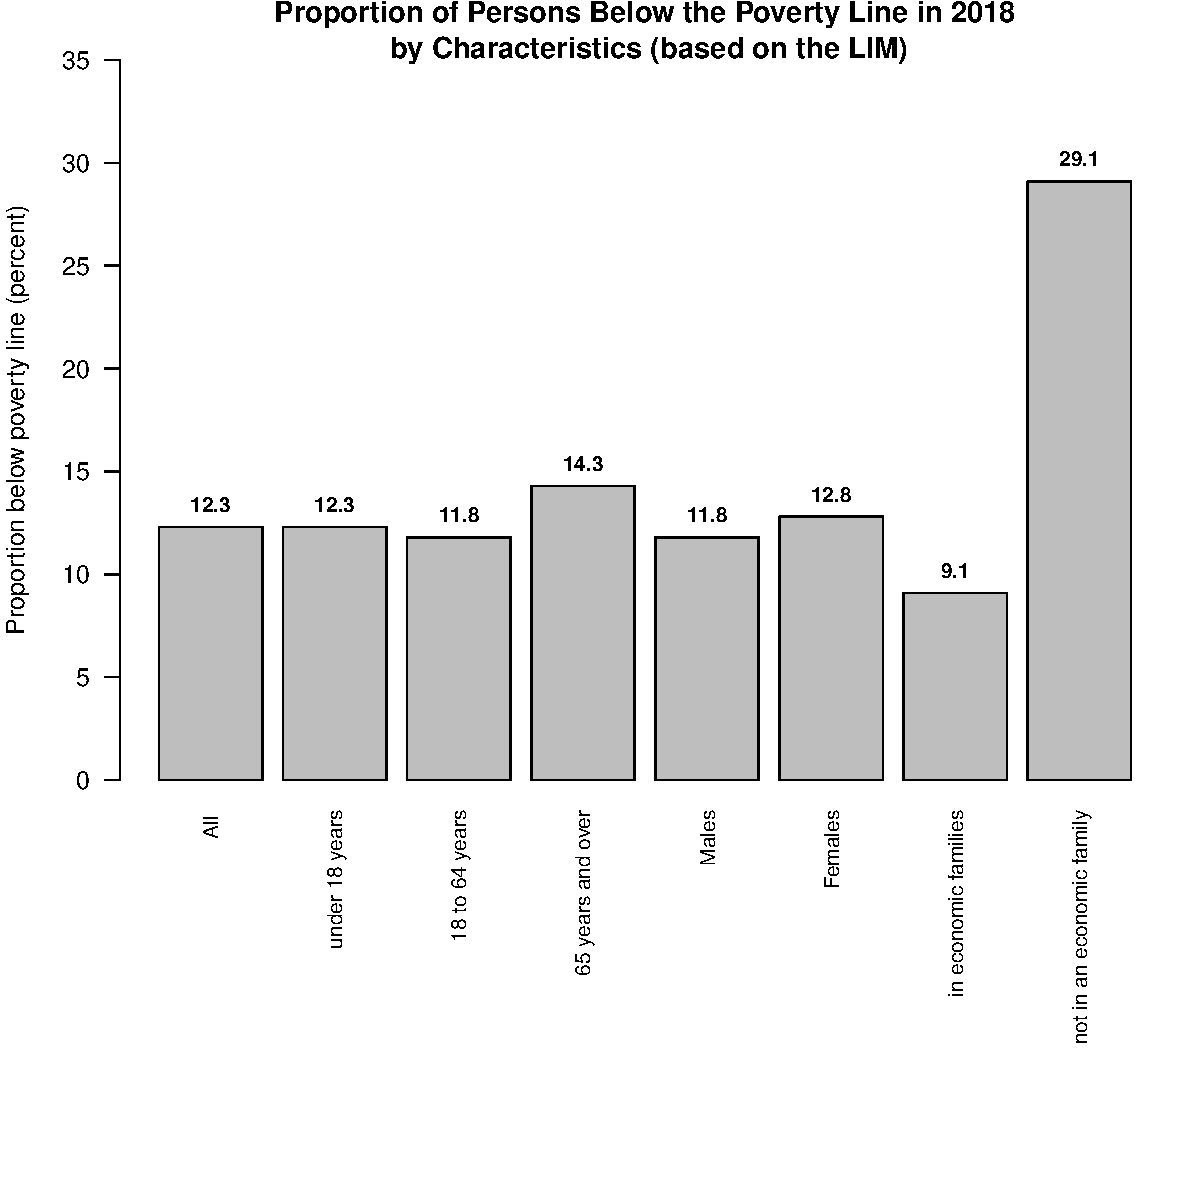
\includegraphics[width=0.6\linewidth]{week7/week7-poverty2-1} 

\end{knitrout}
\end{center}



\subsubsection*{The Poverty Over Time in Canada}

The following graphs show the evolution of poverty in Canada from 1976
to 2018 based on the LIM. The left graph show the evolution for all
person (black solid line), males (dashed red line), females (dotted
green line) and persons in economic families (dot-dashed blue line) and
the right graph shows the evolution for all persons not in family
(black solid line), males not in family (dashed red line) and females
not in family (dotted green line). We separated persons in family from
persons not in family for clarity. 
\begin{center} 
\begin{minipage}{.45\textwidth}
\begin{knitrout}\footnotesize
\definecolor{shadecolor}{rgb}{0.969, 0.969, 0.969}\color{fgcolor}
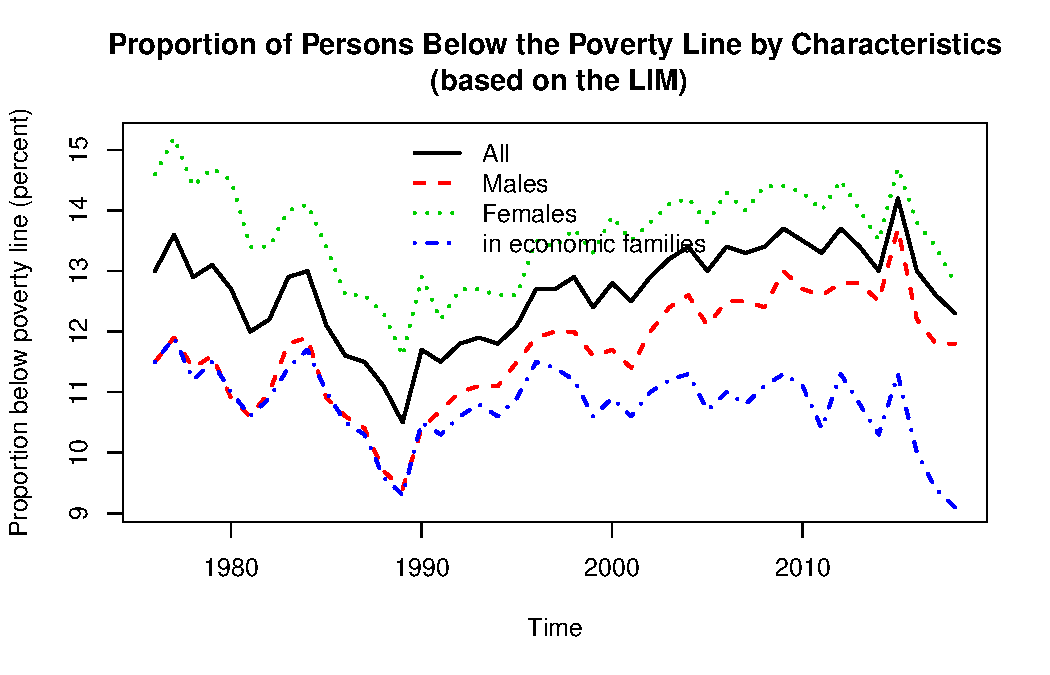
\includegraphics[width=\maxwidth]{week7/week7-poverty3-1} 

\end{knitrout}
\end{minipage}
\begin{minipage}{.45\textwidth}
\begin{knitrout}\footnotesize
\definecolor{shadecolor}{rgb}{0.969, 0.969, 0.969}\color{fgcolor}
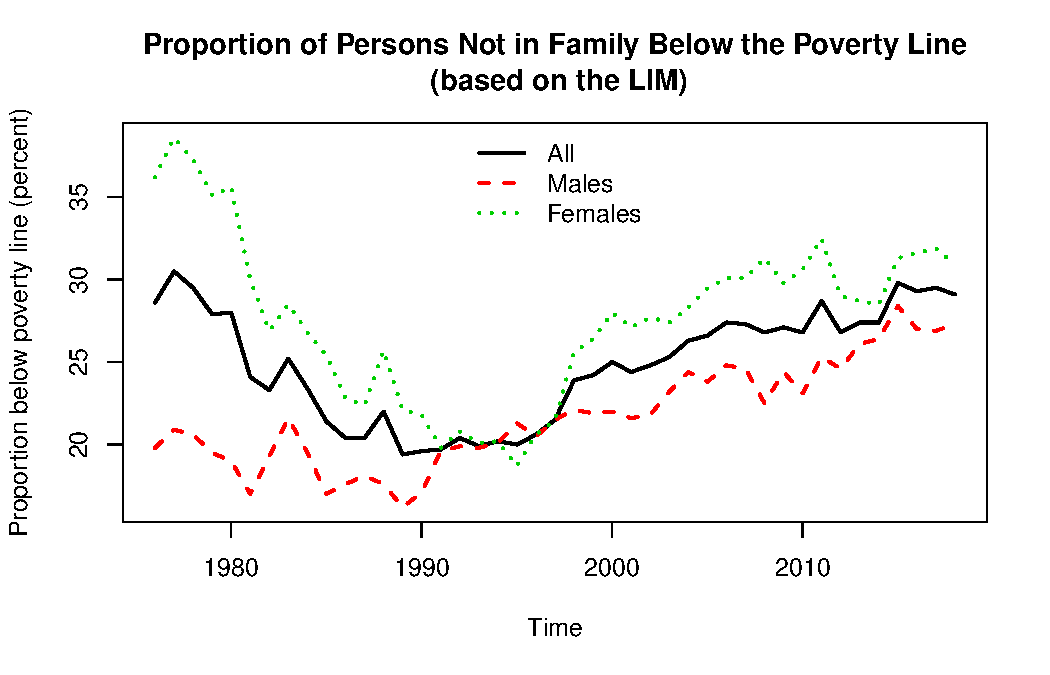
\includegraphics[width=\maxwidth]{week7/week7-poverty4-1} 

\end{knitrout}
\end{minipage}
\end{center}
The overall conclusion is that poverty has decreased from 1976 to 1990
and increased after 1990. The only exception is for the persons in
family for whom poverty has been quite stable over the whole
period. This means that the overall changes in poverty is mostly
driven by the persons not in family. If we compare the situations of
males and females, we can see that the proportion of females below the
poverty line has been systematically higher than the proportion of
males throughout the period. However, the gap is much smaller in 2018
than in 1976, especially for persons not in family: 35\% of females in
1976 compared with 20\% of males and just a few percentage points
difference in 2018.



\begin{important}
Is poverty related to inequality? The simple answer is not
necessarily, because we may have a situation in which everyone is
poor. In this situation, there is no inequality. Similarly, we may
have a situation in which the poorest individual can afford the MBM
and so no individual is below the poverty line. But, this does not
prevent a large portion of the population to be much richer then
others. However, the relationship between poverty and inequality is
more complicated than that. For this course, we will treat poverty and
inequality as two different issues that may or may not be related.
\end{important}

\subsection{Inequality Versus Growth}


In the module readings, you have read about theories that try to
explain the possible relationships between inequality and growth. In
this course, we do not have the theoretical background to understand
those theories. We only want to focus on the empirical evidence. For
example, you will read about the Kuznets hypothesis that predicts that
there is a reversed U-shape relationship between inequality and per
capita real GDP: it starts by being positively related and then
becomes negatively related. Testing such relationships requires
advanced statistical techniques. All we can do in this course is to
verify if we observe such relationship. The data used in this section
is from the World Bank \citep*{gdp-gini-wb}. You can explore the
website and download the data by yourself or use the file
worldData.csv available on the course website.

The data file worldData.csv contains 8 columns: the country names, the
country codes, the most recent year when most variables were
available, the real per capita GDP in thousands of international
dollars of 2011, the Gini coefficients based on after-tax income, the
income share of the bottom 10\% of the income distribution, the income
share of the top 10\% of the distribution and the proportion of the
population that are below the poverty line. The unit of the real GDP
(international dollars of 2011) is a constant price measure that makes
values from different countries comparable. We will learn more about
this in a future  module.

\subsubsection*{Gini Versus Real Per Capita GDP Across Countries}

First, we want to see if we observe a relationship between real per
capita GDP and inequality. The following is the scatter plot of the
Gini as a function of real per capita GDP for the 154 countries
included in the data file for which the two values are available1. For
some selected points, the country codes are written on top.  If you
are not sure which country corresponds to the codes, type ``iso 3166-1
alpha-3 codes'' in any web search engine and you will find a list.

\begin{center}
\begin{knitrout}\footnotesize
\definecolor{shadecolor}{rgb}{0.969, 0.969, 0.969}\color{fgcolor}
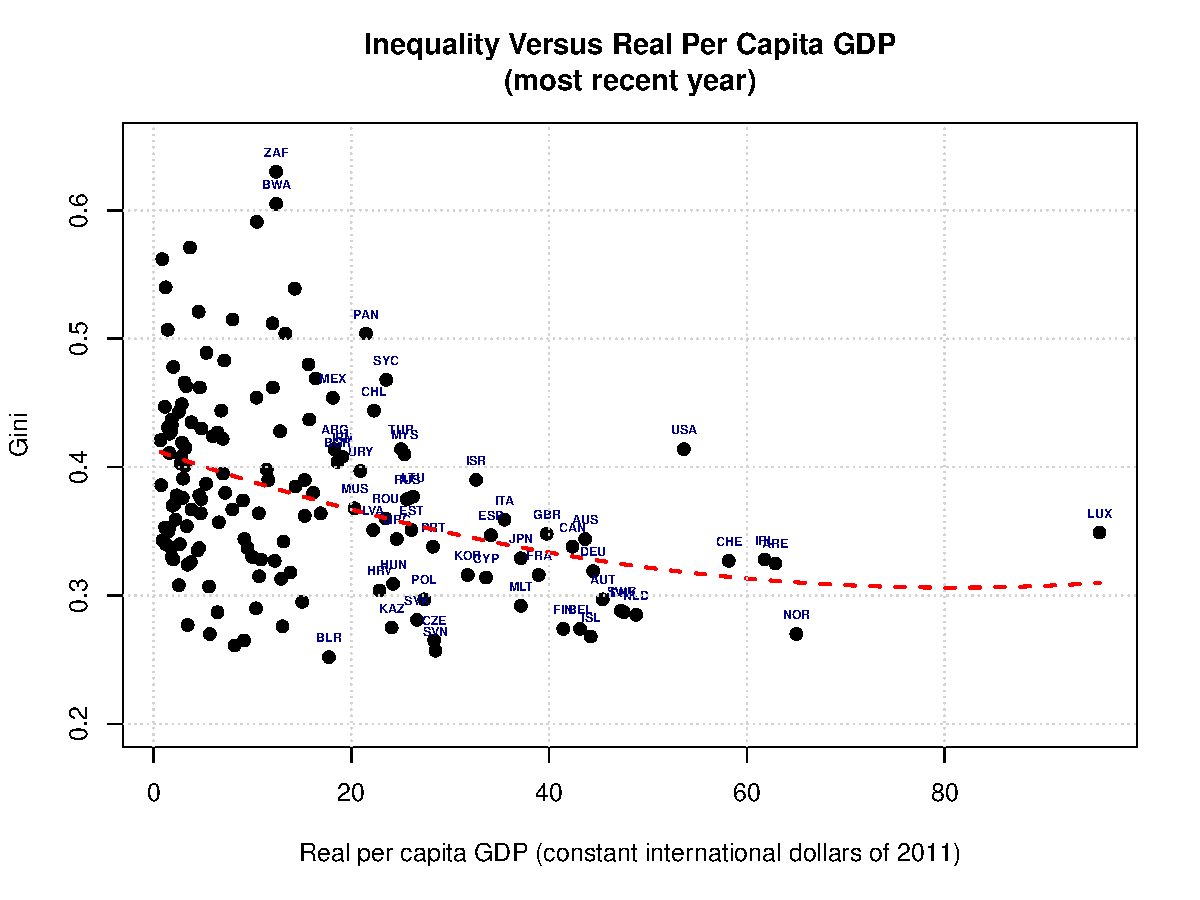
\includegraphics[width=0.7\linewidth]{week7/week7-gdpineq1-1} 

\end{knitrout}
\end{center}
The read dashed line is just to show the average comovement between
inequality and real per capita GDP. We observe a negative relationship
between the Gini coefficient and real per capita GDP which suggest
that richer countries are more equal on average. However, this is only
true on average because there is a lot of variation.  First, we see
that the United States (USA) is more unequal than the average (about
68\% of the countries have a smaller Gini coefficient than the US)
even if it is one of the richest countries. Also, if we look at the
poorest countries (20 thousand and below), we see that the Gini
coefficient is all over the place. The least equal is Belarus (BLR)
with a Gini coefficient of 0.252, and South Africa (ZAF) and Botswana
(BWA) are the most unequal with Gini coefficients of 0.63 and 0.605
respectively. Yet, their per capita DGPs are not that
different. Between them, we see about 108 countries with very
different Gini coefficients. This result shows that poverty and
inequality are not always related.

\subsubsection*{Poverty Versus Inequality}

The following is the scatter plot of the proportion of the population
below the poverty line as a function of the Gini coefficient. In the
data file, this measure of poverty is only available for 125 countries
that are relatively poor (real per capita GDP less than 29
thousand). The red dashed line shows a positive comovement between the
two variables on average. Therefore, there are fewer poor in more
equal countries on average. However, that relationship is not true for
many countries. For example, the proportion of poor in Ukraine is
1.3\% and it is equal to 66.2\% in S\~{a}o Tom\'{e} and Pr\'{i}nciple
(STP), but the two countries have a relatively low Gini
coefficient. On the right side of the graph, we have 17\% of poor in
Namibia (NAM) and 50\% in South Africa (ZAF), and both countries have
similar level of inequality. 

\begin{center}
\begin{knitrout}\footnotesize
\definecolor{shadecolor}{rgb}{0.969, 0.969, 0.969}\color{fgcolor}
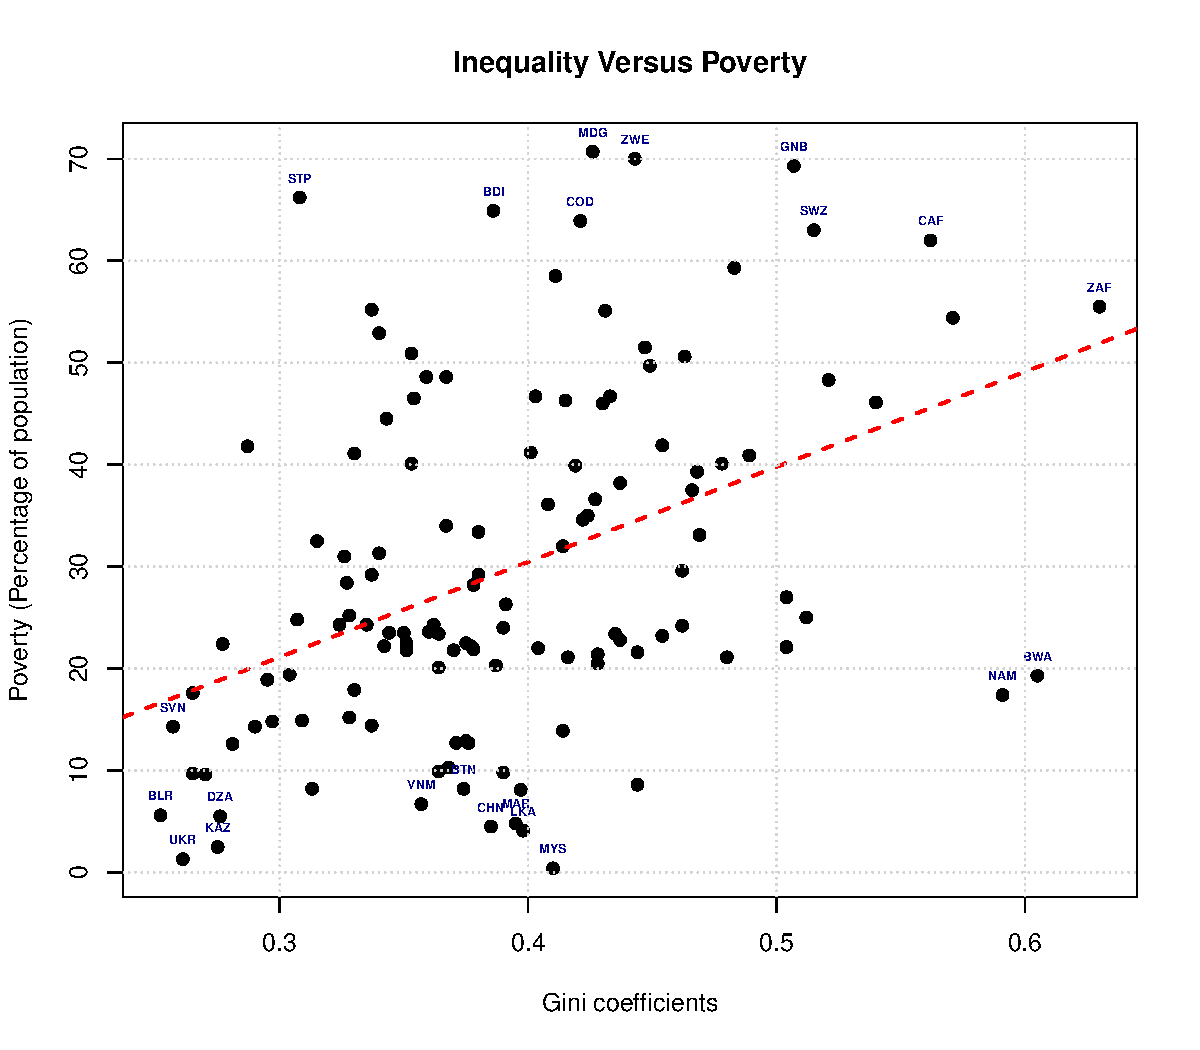
\includegraphics[width=0.7\linewidth]{week7/week7-gdpineq2-1} 

\end{knitrout}
\end{center}


\subsubsection*{Poverty Versus Per Capita GDP}

It is sometimes suggested that growth is the solution to the problem
of poverty. If that's that case, government policies that promote
growth should also help reducing poverty. In this section, we can to
see if we observe a relationship between real per capita GDP and
poverty. In the module readings, there is a scatter plot showing the
relationship between the average income for the bottom quintile and
real per capita GDP. The graph shows that there is a strong positive
comovement between the two variables, which means that the poor get
richer as the economy is growing. We can start this section by
reproducing this graph. We need to compute the average income from the
first decile using the information contained in our data file. The
average income in decile i is given by the following formula:
\[
\mathcolorbox{
\mbox{Average income in decile i} = 10\times\mbox{(Real per capita GDP)}\times 
\mbox{(income share of decile i)}} \,.
\]
\begin{background}
Let $I$ be the total income in the economy, Pop be the population and
$I_i$ be the total income in the i$^\mathrm{th}$ decile. Then, the
average income in decile i is:
\footnotesize
\[
\mbox{Average income in decile i} = \frac{I_i}{Pop/10} = 10\times \frac{I_i}{Pop}\,,
\]
\normalsize
because the population of each decile is 1/10 of the total
population. Using the fact that per capita GDP is $I/Pop$ and the
income share of decile i is $I_i/I$, then 
\footnotesize
\begin{eqnarray*}
  10\times\mbox{(Real per capita GDP)}\times 
\mbox{(income share of decile i)} &=&
10\times\frac{I}{Pop}\times \frac{I_i}{I}\\
& = & 10\times \frac{I_i}{Pop} \\
&=& \mbox{Average income in decile i}
\end{eqnarray*}
\normalsize
\end{background}
Because it is based on GDP, it is equal to the average total income,
not the average after-tax income. Our data file contains the income
share and the real per capita GDP, so we can compute the average
income from the first decile using the formula. The following is the
scatter plot of the two variables. It is clear from the graph that
higher average income implies higher average income for the bottom
10\% of the income distribution. However, the relationship is not
perfect: just compare the United States (USA) with Denmark (DNK) and
Venezuela (VEN) with Belarus (BLR) (same average income but very
different average income for the bottom decile).

\begin{center}
\begin{knitrout}\footnotesize
\definecolor{shadecolor}{rgb}{0.969, 0.969, 0.969}\color{fgcolor}
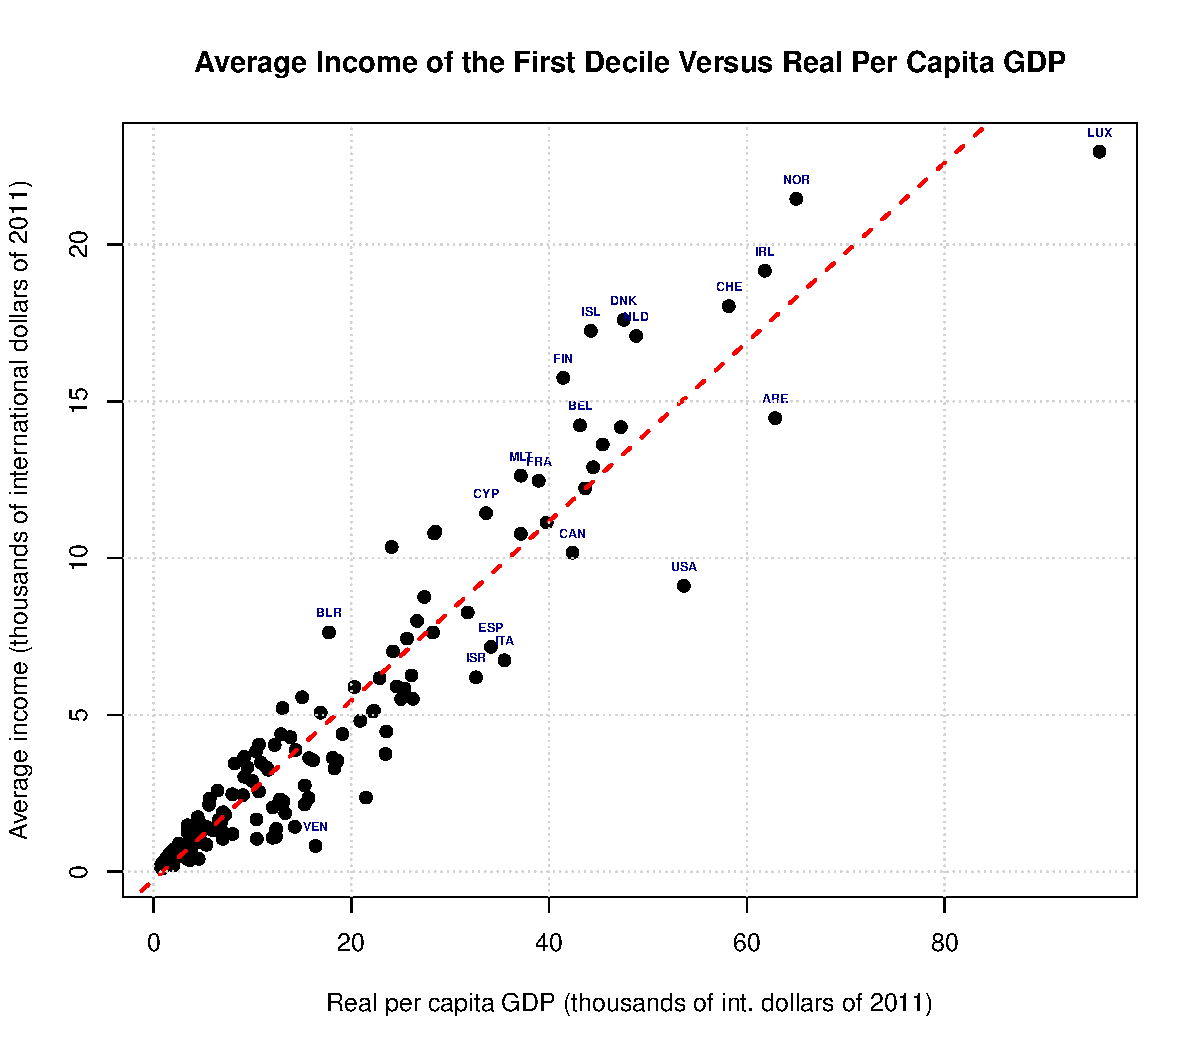
\includegraphics[width=0.6\linewidth]{week7/week7-gdpineq5-1} 

\end{knitrout}
\end{center}

The following graph compares directly poverty with real per capita GDP
using the proportion of the population below the poverty line. On
average (see the red dashed line), the proportion of the population
below the poverty line is lower for countries with higher real per
capita GDP. However, the relationship is not as clear as in the
previous graph. Just compare Eswatini (SWZ) with Ukraine. They both
have the same average income but proportion of poor in Eswatini is
63\% and it is 1.3\% in Ukraine. There is one important factor worth
noticing: the variation gets smaller as average income increases. It
implies that the number of countries with the same average income and
very different proportion of poor gets smaller. This result does
suggest that as real per capita GDP increases, the proportion of poor
becomes low and stable.

\begin{center}
\begin{knitrout}\footnotesize
\definecolor{shadecolor}{rgb}{0.969, 0.969, 0.969}\color{fgcolor}
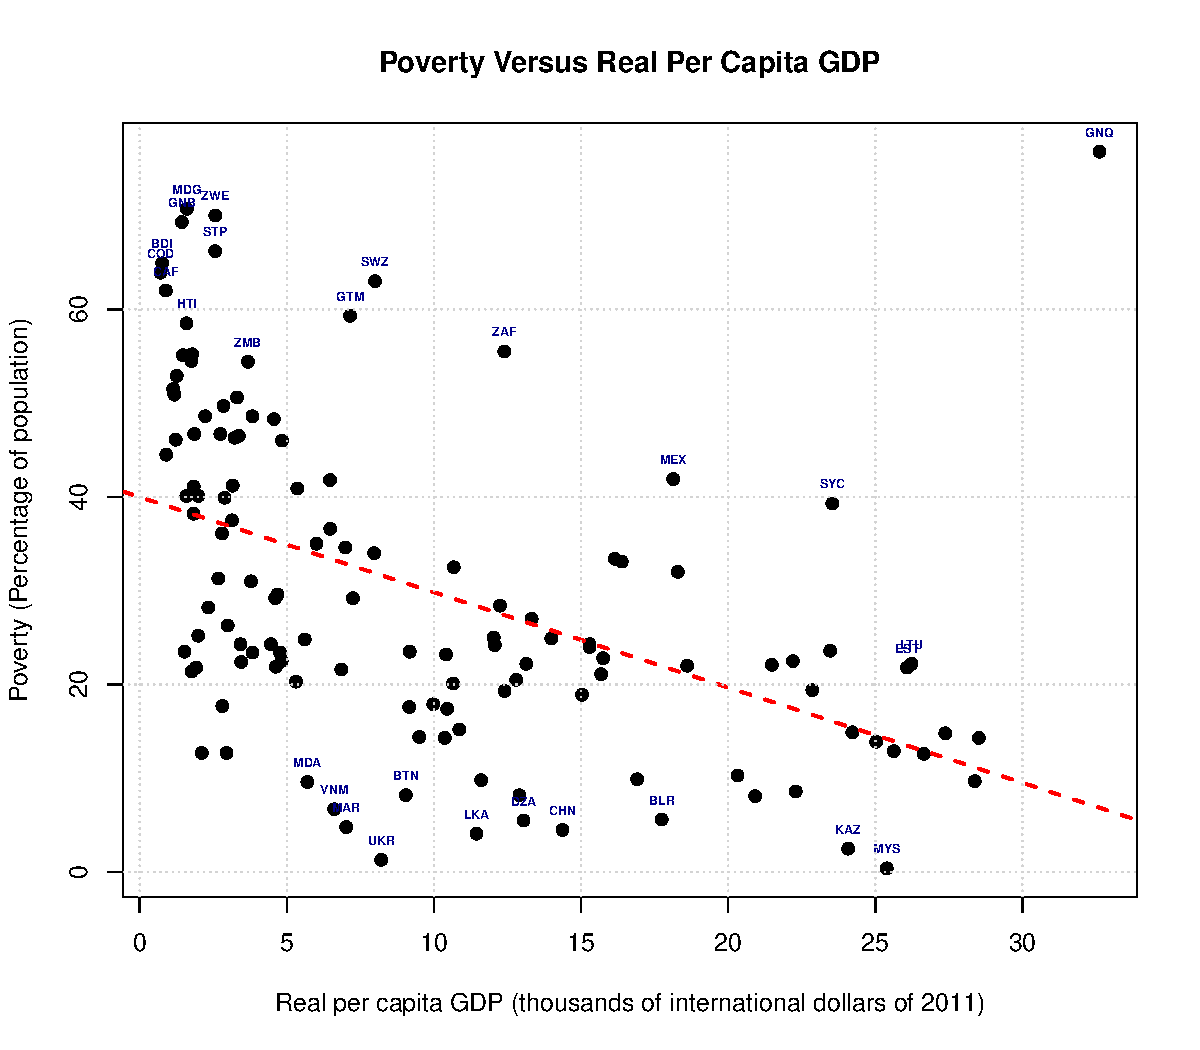
\includegraphics[width=0.6\linewidth]{week7/week7-gdpineq6-1} 

\end{knitrout}
\end{center}

\subsection{Exercise: Poverty versus Per Capita GDP in Canada} 


For this exercise, you need the proportion of persons below the
poverty line (based on the LIM) by characteristics that we used in a
previous section. The series are available in the Statistics Canada
table 11-10-0135-01. You also need the annual real GDP (table
36-10-0222-01) and the annual population (table 17-10-0005-01) series.

In the exercise, try to analyze the relationship between poverty and
real per capital GDP by characteristics. We want to see if the
increase in average income resulted in a reduction in poverty. To
analyze the relationship, use scatter plots and compare: Males and
Females, Males and Females in economic families, and Males and Females
not in economic families.

\subsubsection*{Solution}

The following is the scatter plot of the proportion of persons below
the poverty line (LIM) with respect to the real per capita GDP. The
males are represented by the black circles and the females by the red
triangles. For both series, it seems that higher average income is
associated with a larger proportion of poor.

\begin{center}
\begin{knitrout}\footnotesize
\definecolor{shadecolor}{rgb}{0.969, 0.969, 0.969}\color{fgcolor}
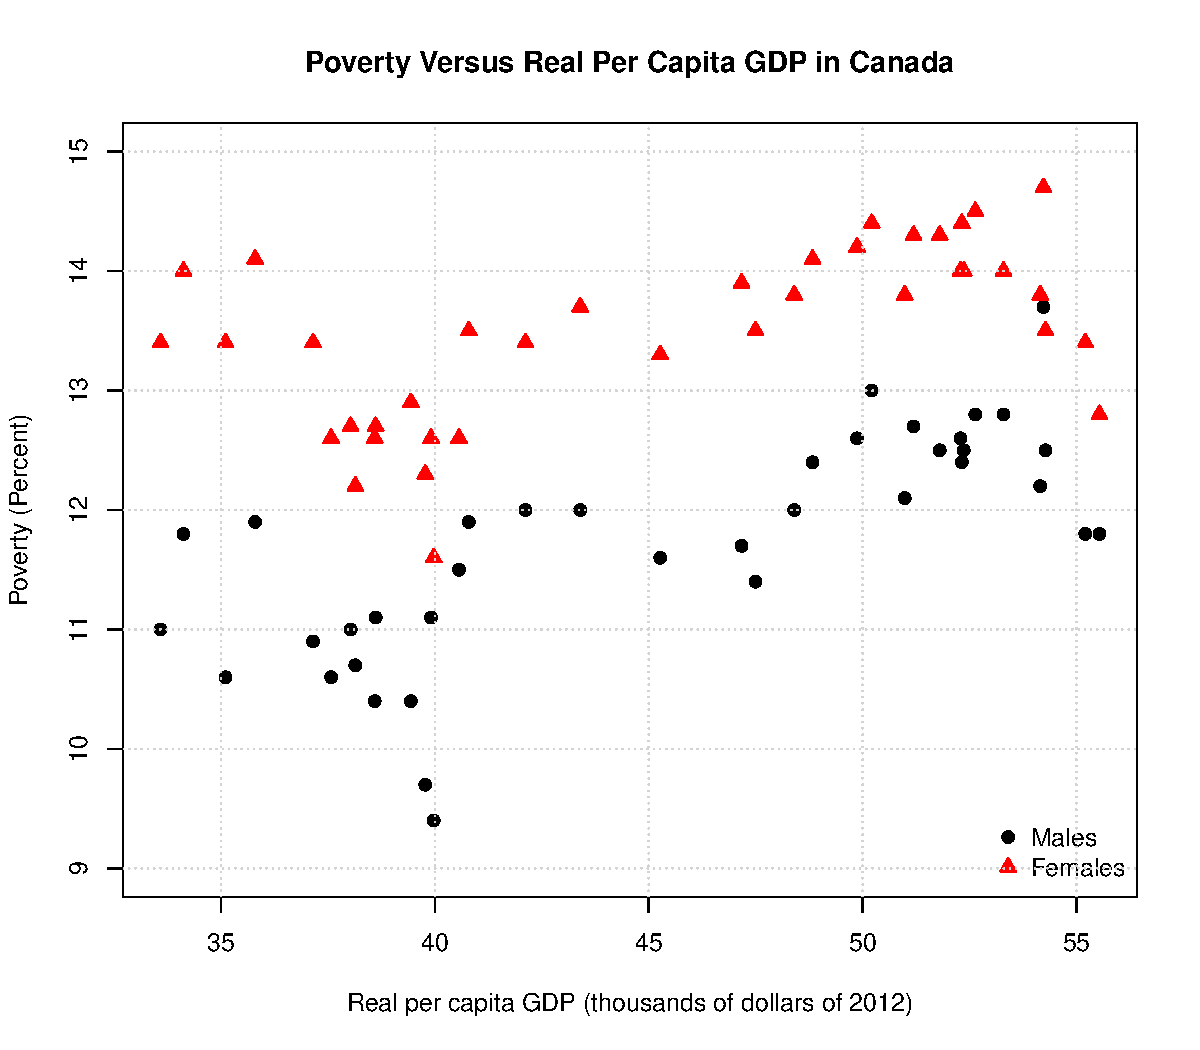
\includegraphics[width=0.6\linewidth]{week7/week7-ex1-1} 

\end{knitrout}
\end{center}

The following is the scatter plot of the proportion of persons below
the poverty line (LIM) with respect to the real per capita GDP for
persons in economic families. The males are represented by the black
circles and the females by the red triangles. For males, there is no
clear relationship between poverty and average income and for females,
higher average income is associated with a lower proportion of
poor. We also observe lots of variation: same average income
associated with different level of poverty.

\begin{center}
\begin{knitrout}\footnotesize
\definecolor{shadecolor}{rgb}{0.969, 0.969, 0.969}\color{fgcolor}
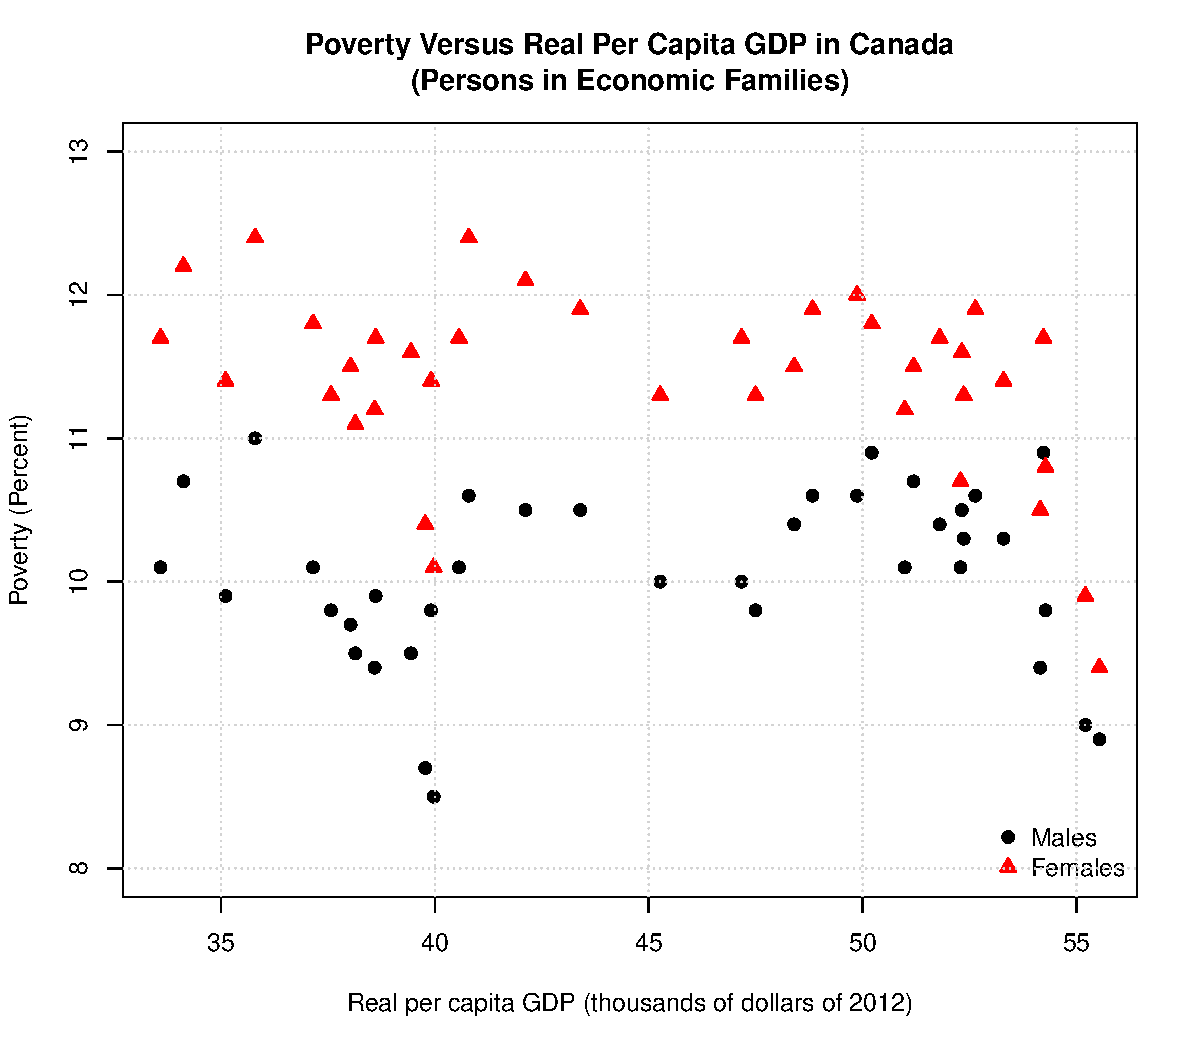
\includegraphics[width=0.6\linewidth]{week7/week7-ex2-1} 

\end{knitrout}
\end{center}

The following is the scatter plot of the proportion of persons below
the poverty line (LIM) with respect to the real per capita GDP for
persons not in economic families. The males are represented by the
black circles and the females by the red triangles. For males, there
is clear positive comovement between the two variables. For females,
we see a negative relationship before real per capita GDP reached 40
thousand dollars of 2012 and a positive relationship after. Overall,
however, it is a positive relationship that we observe. Therefore,
growth does not seem to have solved the problem of poverty for that
group.

\begin{center}
\begin{knitrout}\footnotesize
\definecolor{shadecolor}{rgb}{0.969, 0.969, 0.969}\color{fgcolor}
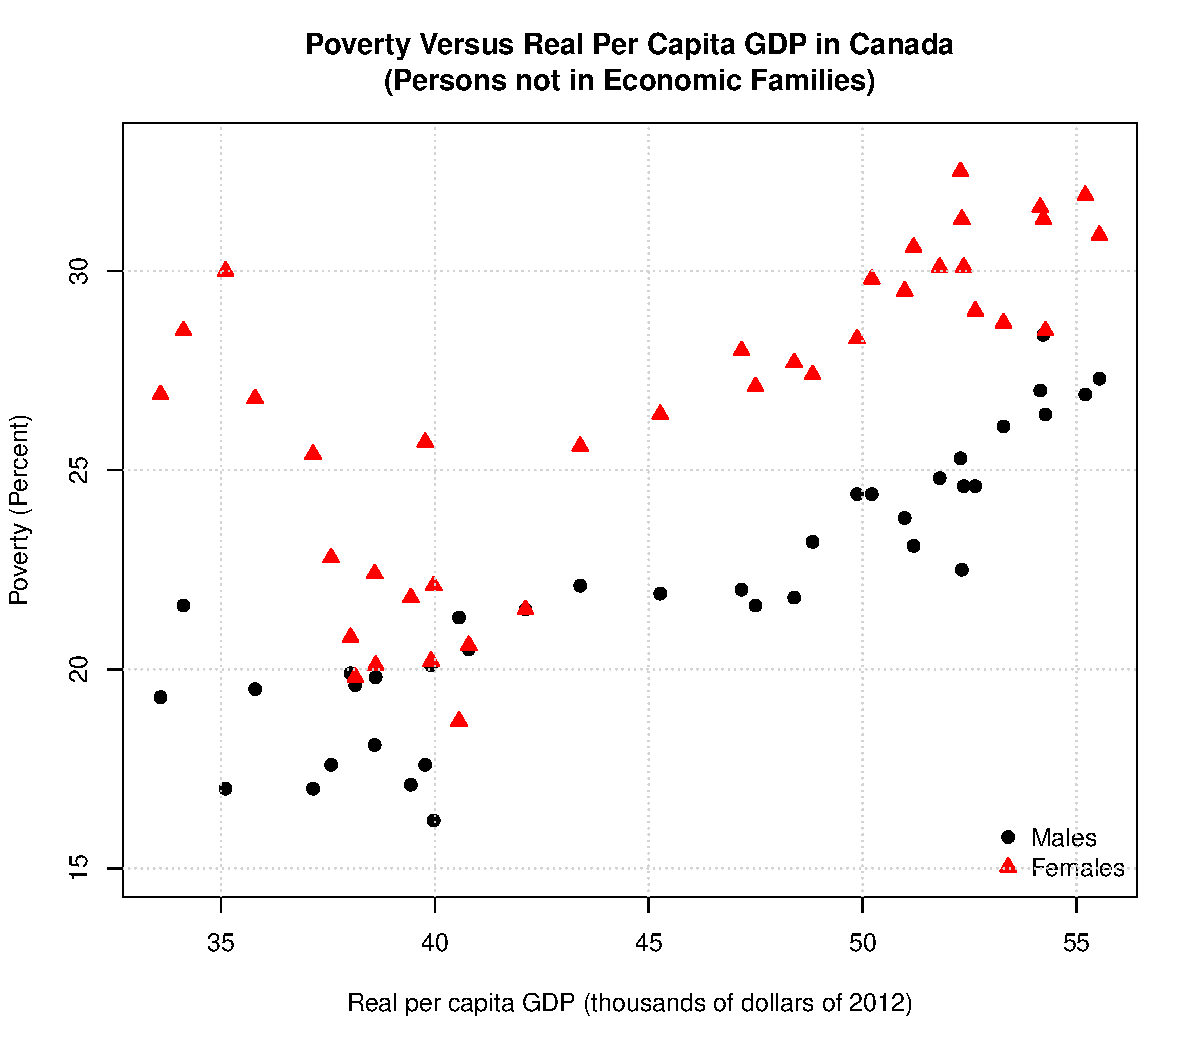
\includegraphics[width=0.6\linewidth]{week7/week7-ex3-1} 

\end{knitrout}
\end{center}
\section{The Sources and Consequences of Inequality}

In this section, we summarize and briefly explain the important points
that you need to remember from the module readings. It is not a
substitute to reading, but a complement to help you identify the
important results.

\subsubsection*{Sources of Inequality}

The following enumerate a few sources of inequality. 
\begin{itemize}
\item Inequality in skills: If some workers have a particular skill
  that is highly in demand, these workers will be well paid compared
  tp the average workers. For example, skilled hockey players will be
  drafted by teams form the national hockey league (NHL) and will be
  paid much more than average workers. As another example, individuals
  with coding skills (software development, data science, etc.) are in
  high demand and therefore well paid compared with unskilled workers.
  This is a natural source of inequality that can hardly be
  controlled.
\item Inequality in how skills are valued: Depending on how the
  society values products and services, some skills may result in
  higher income than others. It also depends on the demand and supply
  of those skills: if a particular skill is in high demand and low
  supply, it will be more valued. 
\item Inequality in education: We assume here that higher education
  leads to higher income. The following compares the median wage by
  level of education in 2016 \citep*{educ-wage}.
\begin{center}  
\resizebox{0.9\linewidth}{!}{  
\begin{tabular}{lcccc}
&  \multicolumn{4}{P{15cm}}{\textbf{Median annual earnings of women and men aged 25 to 64 who worked full time and full year as paid employees}}\\\hline
&High school diploma&Apprenticeship certificate&College diploma&Bachelor's degree\\
Women&  \$43,254&\$38,230&\$48,599&\$68,342\\
Men&  \$55,774&\$72,955&\$67,965&\$82,082\\\hline
\end{tabular}}
\end{center}
From the table, more educated workers earn more: a gap of about
\$25,000 between high school diploma and bachelor's degree. Therefore,
inequality of education is likely to create income inequality. Notice
that education inequality across countries is also a source of income
inequality in the world. Therefore, government policies that focus on
reducing education inequality is likely to also reduce income
inequality.
\item Technological advances: This source is related to skills and
  education. For example, advances in information technology increases
  the value of computer scientists without affecting the value the
  unskilled workers or other type of unrelated skilled workers. For
  example, we saw in previous section that the Gini coefficient in
  Canada increased substantially in the '90s, a period characterized
  by a boom in computer technology.
\item Value of education: Everything that affects the value of being
  educated will increase the impact of education inequality on income
  inequality. For example, technological advances affect the value of
  some types of education.   
\end{itemize}
This is a short list of what may cause income inequality. We will
cover other sources in more details in the Growth and Development
module.

\subsubsection*{The Effect of Inequality on Growth}

Explaining the effect of inequality on growth requires theoretical
background that we don't have, and testing empirically whether this
relationship exists is something difficult even for well trained
economists. The following quote from the readings summarizes well the
issue:

\say{Does inequality raise or lower growth?  Unfortunately, available
  statistical data are unable to answer this question. Although some
  economists claim to find evidence that inequality is on average bad
  for growth, others claim the data point in the opposite direction.}

Just to mention the possible channels through which inequality may have
an effect of growth, the inequality may affect:

\begin{itemize}
\item investment, which affects growth through its impact on the
  accumulation of capital goods (goods used to produce),
\item education, which affects the productivity of workers,
\item taxation (for redistribution purposes), which effects incentives
  to work or produce,
\item the political stability, which affects the incentive to invest, and
\item the level of criminality, which implies wasting resources to
  prevent it instead of producing goods.
\end{itemize}

Most economists think that those channels exist, but we don't know
which one has the largest impact. For this course, you need to
understand the intuition behind the different channels, and be aware
of the difficulty of evaluating their relative impact.

\begin{important}
Only read the sub-section Empirical Evidence from the Effect of Income
Inequality on Economic Growth section of the module readings. In
particular, the historical evidence from Latin America, the United
States and Canada at the end of the sub-section is a clear and
intuitive description of how inequality may lead to lower growth.

You may read the other sections for own interest, but it is not
required for the course. They require too much theoretical background.
  \end{important}

\subsubsection*{Economic Mobility}

Economic mobility is defined as the ability for individuals to move
from one part of the income distribution to another (e.g. moving from
the first quintile to the second of third quintile). This is much
harder to measure than inequality. In the last section of the module
readings, we see a transition matrix which is a way to measure
mobility. For example, we see that persons whose parents were in the
bottom quintile of the income distribution have 42\% chance of being
in the bottom decile, 23\% chance of being in the second and 6\%
chance of being in the top decile.  Also, persons whose parents are in
the third quintile have almost equal chance to be in any
quintile. This is a sign that there is some mobility in the
economy. One main advantage of living in a highly mobile economy is
that every one has equal chance of being successful. In absence of
mobility, poor families would remain poor for generations.

Two important factors that affect mobility are:

\begin{itemize}
\item The accessibility of education: Children whose parents are poor have
  more chance to be in higher deciles if education is easily
  accessible.
\item The accessibility of health care: Health has an impact on school
  performance. Therefore, having an accessible health system helps
  poor children to acquire a higher level of education and move to a
  higher income decile than their parents.    
\end{itemize}

\newpage

\bibliography{econ102}

\end{document}
